% !TeX program = xelatex
\RequirePackage{fix-cm}
\documentclass[UTF8,a4paper,zihao=-4,fontset=none,scheme=plain]{ctexart}
\usepackage[top=3.2cm,bottom=2.54cm,left=3.175cm,right=3.175cm,headheight=14mm,headsep=3mm]{geometry}
\usepackage{amsmath,booktabs,tabularx,array,graphicx,tikz,float,placeins}
\usepackage{caption}
\usepackage{fancyhdr}
\usepackage[hidelinks]{hyperref}
\usetikzlibrary{arrows.meta,positioning}
\setmainfont{Times New Roman}
\setCJKmainfont[AutoFakeBold=2]{SimSun}
\setCJKsansfont{SimHei}
\setCJKmonofont{FangSong}
\setCJKfamilyfont{zhsong}[AutoFakeBold=2]{SimSun}
\newcommand{\songti}{\CJKfamily{zhsong}}
\ctexset{
 section={name={第,部分},number=\chinese{section},afterindent=true,
   format=\songti\bfseries\fontsize{14bp}{21bp}\selectfont,
   aftername=\quad,beforeskip=12bp,afterskip=6bp},
 subsection={afterindent=true,format=\songti\bfseries\fontsize{12bp}{18bp}\selectfont,
   aftername=\quad,beforeskip=9bp,afterskip=4bp},
 subsubsection={afterindent=true,format=\songti\bfseries\fontsize{12bp}{18bp}\selectfont,
   aftername=\quad,beforeskip=6bp,afterskip=3bp}
}
\setlength{\parindent}{2em}
\setlength{\parskip}{0pt}
\setlength{\emergencystretch}{1em}
\AtBeginDocument{\songti\fontsize{12bp}{18bp}\selectfont}
\renewcommand{\figurename}{图}
\renewcommand{\tablename}{表}
\captionsetup{font=small,labelfont=bf,labelsep=quad,skip=6bp}
\renewcommand{\arraystretch}{1.25}
\setlength{\tabcolsep}{5pt}
\newcolumntype{Y}{>{\raggedright\arraybackslash}X}
\tikzset{block/.style={draw,align=center,minimum height=10mm,
 text width=29mm,font=\small,inner sep=3pt},
 flow/.style={-{Stealth[length=2mm]},thick}}
\pagestyle{fancy}
\fancyhf{}
\fancyhead[C]{
\includegraphics[width=65.16mm]{images/competition-header.png}}
\fancyfoot[C]{\thepage}
\renewcommand{\headrulewidth}{0.75pt}
\renewcommand{\footrulewidth}{0pt}



\begin{document}
\begin{center}
 {\bfseries\fontsize{18bp}{27bp}\selectfont
 基于FPGA与RISC-V的多模态\\室内照护与跌倒预警终端\par}
\end{center}

\section*{摘要}
针对室内照护中短暂姿态变化与持续异常难以区分、无人时持续检测产生冗余开销的问题，设计并实现了一种基于FPGA与RISC-V的多模态室内照护与跌倒预警终端。FPGA完成全视场图像缩小、视频输出和执行器时序控制，RISC-V调度INT8人体检测模型，结合目标ID、框形变化及帧差运动维护人员状态。预警采用“正常—疑似—预警”三级状态，同一目标疑似状态持续10秒后升级为红色，并触发事件记录及模拟照护响应。常规监测以视觉为主，红外在近距离、空间配准与热观测有效时辅助排除人物照片干扰；远距离热像分辨能力受限，辅助信息不足时沿用纯视觉判断。

针对持续无人场景，系统以统一状态协调推理、显示和传输：降低完整检测调用频率，调暗HDMI背景，将Web预览发送目标由10 FPS降至2 FPS，同时保留运动检查和周期检测，支持人员重新进入后恢复。风险事件关联目标信息及同帧缩略图，经Web复核、电脑存档与外部消息服务连接现场响应和远程查看。系统通过QQ消息桥接接入国产大模型DeepSeek，提供活动概述与照护问答，构成板端实时判断与电脑端语言交互的协同架构。

实物演示展示了双人检测、正常蹲下与持续疑似的分阶段处理、无人监视与入场恢复，以及模拟门联动。地面位置经四点映射后，在网页地图与实体灯板上显示当前位置和短时轨迹；手机端展示活动问答。硬件实现使用60,114个XLR、255个片内RAM块和75个DSP，建立与保持时序余量均为正。结果表明，系统实现了本地感知、持续风险判断、位置表达与远程复核的协同；识别增益和整机节能收益仍需量化评价。

\par\vspace{12bp}
\noindent\textbf{关键词：}智能家居；多模态照护；分阶段跌倒预警；轨迹可视化；大模型交互

\clearpage
\section{作品概述}
\subsection{功能与特性}
室内照护终端既需要发现异常人员，也需要判断异常是否持续，并将风险传递给能够采取行动的照护人员。本作品“智龄卫士”围绕这一需求，将图像采集、人体检测、目标关联、分阶段预警和照护响应组织为连续流程。视觉分支提供人员位置及动作变化，红外阵列和温湿度传感器提供区域热分布及环境信息，风险决策在板端完成。

系统提供单人主目标与多人跟踪两种模式，以16个轨迹槽保存人员短时历史。正常、黄色疑似和红色预警表示不同风险阶段；网页地图和实体灯板表达选定主目标的位置与短时轨迹，救援模块检查有效目标中的红色风险。Web提供实时查看、事件回看、CSV导出和人工干预；电脑辅助程序承担视频转换、历史存档、消息通知及语音桥接，并通过QQ接入国产大模型DeepSeek，支持面向照护人员的自然语言问答。模拟门验证预警后的执行响应。

\subsection{应用领域}
作品面向固定机位的居家照护、养老空间巡视及嵌入式人工智能教学。固定安装便于建立图像与地面位置的映射关系，现场提示及远程记录便于照护人员发现异常并复核。系统输出辅助风险提示，处置仍需结合现场情况；模拟门承担响应流程演示。

\subsection{主要技术特点}
系统采用\textbf{连续数据通路与状态控制分工}的实现方式。FPGA负责像素流预处理和严格输出时序，RISC-V负责模型调度、人员历史及协议服务，DDR保存图像、事件和灯帧。全视场缩小适配96×96输入，保留画面边缘及近地面区域。

感知结果分别保存为RGB候选、热辅助确认和风险状态：候选用于目标关联，热特征补充目标属性，预警依据同一人员的连续状态推进。无人轻量监视由统一状态同步调整检测、显示及预览，事件通过同帧缩略图、入库确认和有限队列补传支持复核。各模块围绕同一目标及事件协同工作。

\subsection{主要性能指标}
表\ref{tab:overview}列出主要配置；采集配置与预览目标均不代表端到端处理帧率。
\begin{table}[H]
 \centering\small
 \caption{主要性能与配置}\label{tab:overview}
 \begin{tabularx}{.94\linewidth}{@{}p{28mm}>{\centering\arraybackslash}X@{}}
 \toprule 项目 & 配置 \\
 \midrule
 图像采集 & 1920×1080，30 FPS \\
 检测模型 & 96×96×3，INT8 \\
 目标跟踪 & 16个轨迹槽 \\
 红外与环境 & 32×24热阵列、温湿度 \\
 持续预警 & 同ID疑似持续10秒 \\
 Web预览 & 320×180，目标10／2 FPS \\
 灯光输出 & 256矩阵＋28外墙＋4预留 \\
 硬件资源 & XLR 60,114；RAM块255；DSP 75 \\
 \bottomrule
 \end{tabularx}
\end{table}

\subsection{主要创新点}
（1）\textbf{持续风险判断：}关联人员ID、姿态和运动历史，同目标疑似持续10秒后升级预警。

（2）\textbf{无人协同调度：}统一降低推理与预览频率、调暗显示，保留运动唤醒和周期检测。

（3）\textbf{智能家居联动：}融合视觉、红外及环境信息，联动轨迹灯板、模拟门与远程提醒。

（4）\textbf{国产大模型交互：}经QQ桥接接入DeepSeek，提供照护问答，板端独立报警。

\subsection{设计流程}
设计首先从覆盖范围、持续异常判断、无人冗余和照护响应四项需求确定流程，再划分FPGA、RISC-V与电脑辅助程序的任务。硬件阶段完成图像、传感器、DDR及输出接口；软件阶段依次连接模型推理、目标关联、风险状态、场景调度和事件服务。功能验证覆盖双人进入、真人与照片对照、正常蹲下、持续疑似、无人入场切换、行走轨迹及手机问答，资源与时序依据硬件实现报告评价。

\FloatBarrier
\clearpage
\section{系统组成及功能说明}
\subsection{整体介绍}
系统按“感知输入—板端判断—照护输出—事件复核”组织，结构见图\ref{fig:architecture}。FPGA承担连续像素处理、视频输出及执行器时序，RISC-V承担模型调度、目标关联、风险状态和通信服务\cite{project}。电脑提供视频转换、数据库及外部通知接口。风险由板端生成，电脑扩展查看和通知能力，二者通过视频、状态与事件三类数据连接。

\begin{figure}[H]
 \centering
 \begin{tikzpicture}[node distance=6mm]
  \node[block,text width=52mm] (fpga) at (0,0) {FPGA：摄像头与像素流\\全视场缩小／TinyML加速接口\\HDMI／UDP预览／执行器时序};
  \node[block,text width=52mm] (cpu) at (7,0) {RISC-V：INT8模型调度\\RGB关联、辅助确认、风险状态\\HTTP／TCP事件／无人调度};
  \node[block,text width=52mm] (sensor) at (0,-2.3) {红外阵列／温湿度\\I\textsuperscript{2}C采集、缓冲与时间标记};
  \node[block,text width=52mm] (act) at (7,-2.3) {板端照护输出\\DDR灯帧→FPGA流式发送\\位置灯板／外墙灯／模拟门};
  \node[block,text width=52mm] (pc) at (0,-4.6) {电脑辅助：UDP→MJPEG\\TCP接收→SQLite存档\\UART语音桥／HTTP事件监测};
  \node[block,text width=52mm] (user) at (7,-4.6) {浏览器与外部通知\\板载页面＋电脑视频／历史\\QQ提醒；DeepSeek照护问答};
  \draw[flow] (fpga)--node[above,font=\scriptsize]{帧／控制}(cpu);
  \draw[flow] (sensor.north east)--(cpu.south west);
  \draw[flow] (cpu)--(act);
  \draw[flow] (fpga.west)--++(-.4,0)|-(pc.west);
  \draw[flow] (cpu.east)--++(.5,0)|-(user.east);
  \draw[flow] (pc)--(user);
  \draw[flow,dashed] (user.north west)--(act.south west);
 \end{tikzpicture}
 \caption{系统总体数据与控制关系}\label{fig:architecture}
\end{figure}

实时预览与事件记录采用不同通路：FPGA通过UDP发送预览，RISC-V通过HTTP发布状态及控制接口，并通过TCP上报事件。预览用于持续查看，事件用于保存触发依据；每条事件绑定目标ID、采集时间、检测框和同帧缩略图。传感器记录采样时间，目标热查询同时检查跨传感器空间关系，使连续画面、离散事件与辅助热观测各自具有明确用途。

\subsection{硬件系统介绍}
\subsubsection{硬件整体介绍}
硬件平台采用Ti60F225I3开发板，集成RISC-V软核、TinyML相关硬件和DDR资源\cite{board,tinyml}。SC431HAI通过MIPI输入图像\cite{camera}，MLX90640和SHT30通过I\textsuperscript{2}C提供热阵列与环境数据。连续像素处理及输出波形放在FPGA中，目标历史、事件和灯帧使用DDR，片内RAM用于访问时序要求较高的数据通路。主要分工见表\ref{tab:modules}。
\begin{table}[H]
 \centering\small
 \caption{系统模块与任务分工}\label{tab:modules}
 \begin{tabularx}{\linewidth}{@{}p{26mm}Y Y@{}}
 \toprule 模块 & 主要任务 & 设计特点 \\
 \midrule
 FPGA视频及接口 & ISP、区域缩小、HDMI、UDP及执行器波形 & 连续像素流与硬件时序处理 \\
 RISC-V与TinyML & 模型调度、目标关联、热查询与风险判断 & 维护目标历史及照护状态 \\
 红外与环境传感 & 热阵列、温湿度及采集时间信息 & 提供区域热观测与环境参考 \\
 DDR灯帧与输出 & 灯帧暂存与握手供数 & 分离完整帧存储与串行波形生成 \\
 电脑辅助工具 & MJPEG、SQLite、QQ及UART语音 & 预览、存档和外部通知 \\
 \bottomrule
 \end{tabularx}
\end{table}

\subsubsection{机械设计介绍}
终端由开发平台、摄像头、传感器外壳及照护演示机构组成，采用3D打印外壳组织安装。前部为摄像头和传感器保留观测开口，背部设置通风孔及连接接口。摄像头与热阵列固定安装，高度、俯仰角及工作距离共同决定覆盖范围。位置显示通过地面四点标定建立图像与平面地图的对应关系，RGB与红外配准另用独立参数建立跨传感器映射，两种标定分别服务于地面定位和目标区域热查询。

外壳前、后视实物见图\ref{fig:mechanical-layout}。感知组件集中在前部支架，后部通风孔及接口开口对应板卡散热与连接需求，底板承载板卡和支架；外壳实物的正面与斜视图见图\ref{fig:enclosure-views}。
\begin{figure}[H]
 \centering
 \begin{minipage}[t]{.48\linewidth}
  \centering
  \parbox[c][45mm][c]{\linewidth}{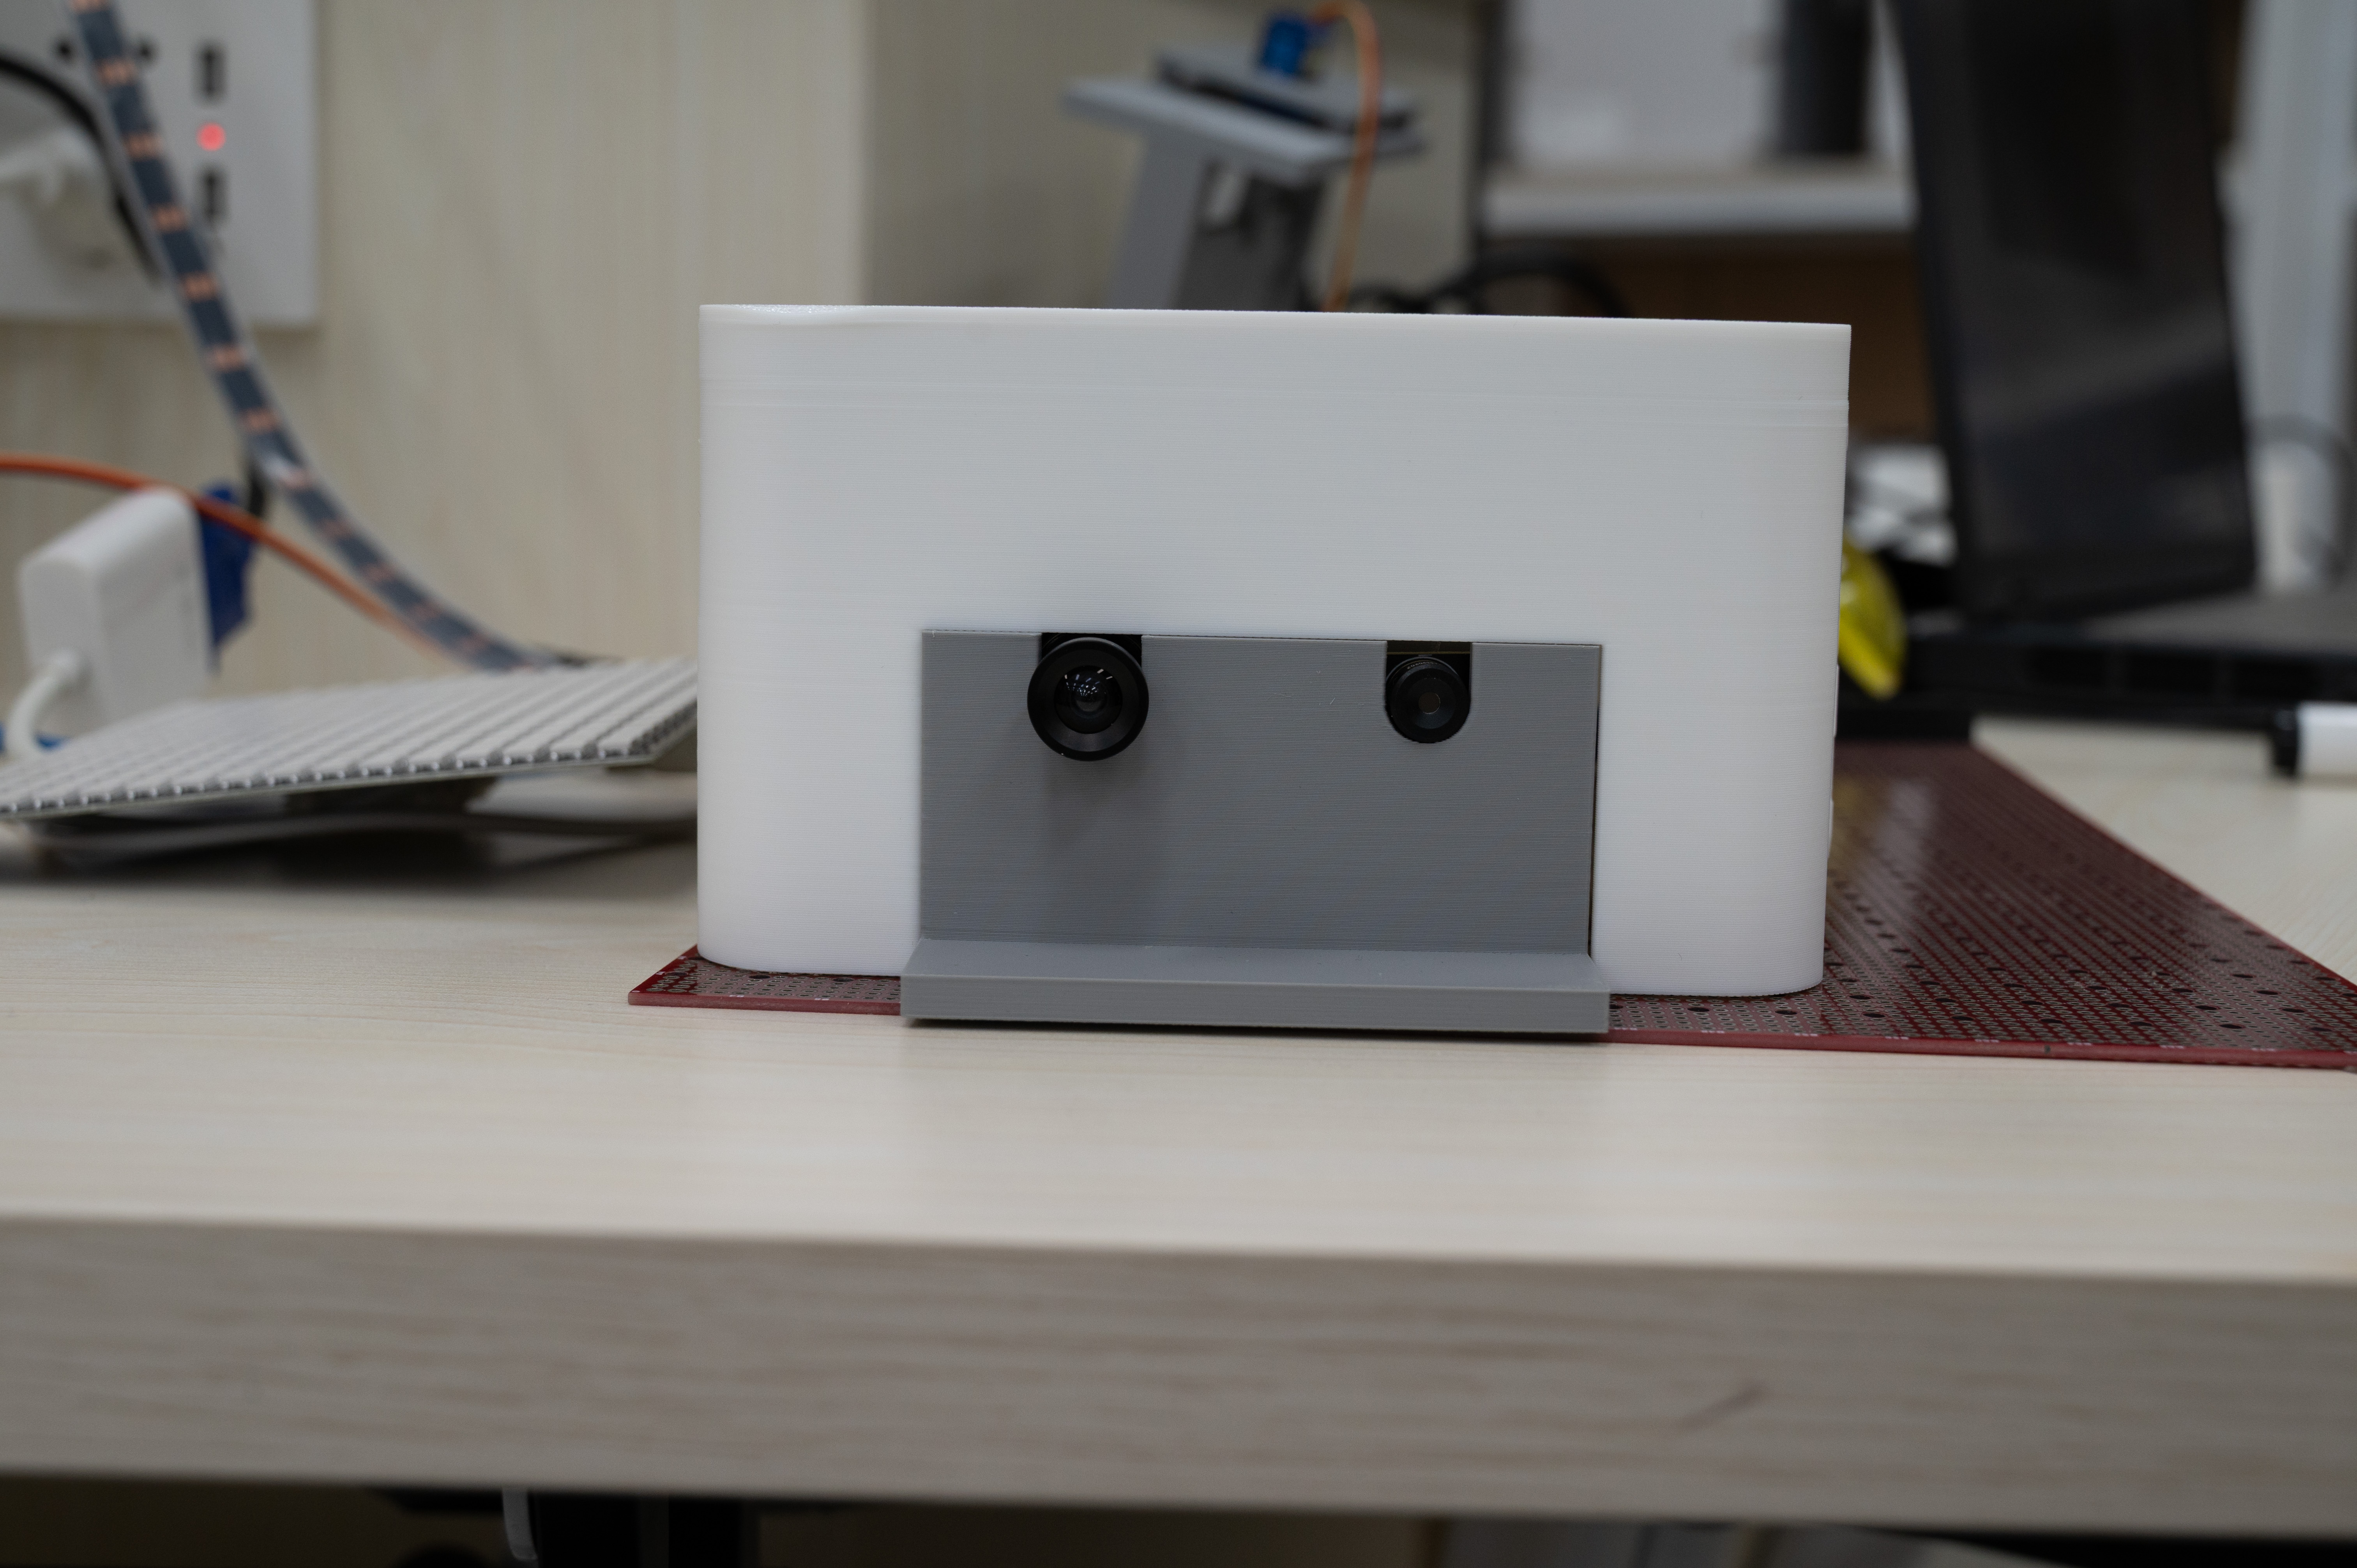
\includegraphics[width=\linewidth,trim=134mm 104mm 80mm 55mm,clip]{images/enclosure-front-photo.jpg}}
  \par\small（a）前部观测面
 \end{minipage}\hfill
 \begin{minipage}[t]{.48\linewidth}
  \centering
  \parbox[c][45mm][c]{\linewidth}{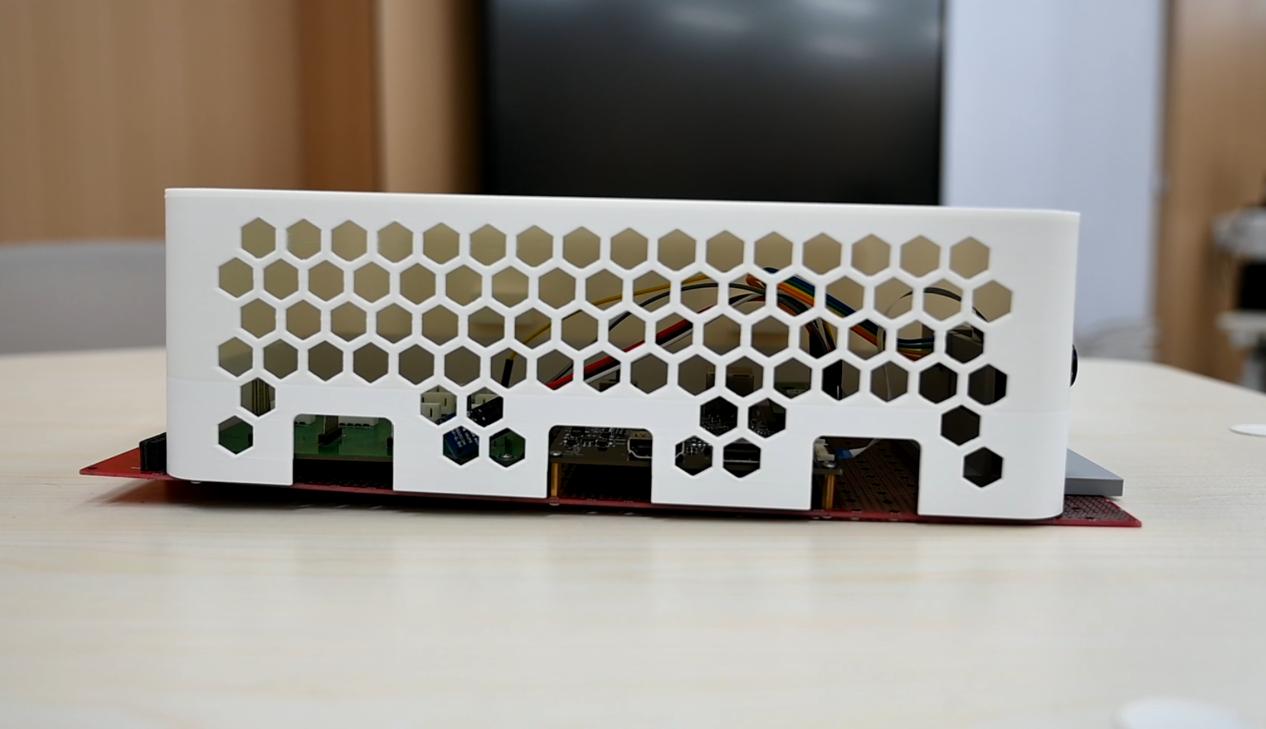
\includegraphics[width=\linewidth,trim=11mm 31mm 18mm 28mm,clip]{images/enclosure-rear-photo.png}}
  \par\small（b）后部通风与接口面
 \end{minipage}
 \caption{终端外壳前、后视实物}\label{fig:mechanical-layout}
\end{figure}

\subsubsection{电路各模块介绍}
\textbf{接口与引脚配置。}
系统将摄像头、视频显示和网络连接保留在开发板原有接口，红外、温湿度及执行器接入扩展排针。表\ref{tab:external-pins}列出外接部件的工程端口、FPGA封装球位和排针编号，表\ref{tab:onboard-pins}列出板载主要接口的信号分配。球位与方向依据工程接口约束及实现后的引脚报告核对，J7扩展口经转接子卡连接至J28同编号排针，编号对应开发板说明书第6.2、6.3节\cite{board,project}。

\begin{table}[H]
 \centering\small
 \caption{外接传感器与执行器引脚配置}\label{tab:external-pins}
 \begingroup
 \newcommand{\pincell}[1]{\begingroup\renewcommand{\arraystretch}{1}\begin{tabular}[c]{@{}c@{}}#1\end{tabular}\endgroup}
 \setlength{\tabcolsep}{3pt}
 \begin{tabularx}{.94\linewidth}{@{}>{\centering\arraybackslash}p{22mm}>{\centering\arraybackslash}p{29mm}>{\centering\arraybackslash}p{29mm}>{\centering\arraybackslash}p{14mm}>{\centering\arraybackslash}X@{}}
 \toprule 部件与信号 & 工程端口 & \pincell{FPGA球位\\及GPIO名称} & \pincell{J28\\针号} & \pincell{方向及\\I/O电压} \\
 \midrule
 \pincell{MLX90640\\I\textsuperscript{2}C时钟} & \texttt{mlx\_scl} & \pincell{C5\\\texttt{GPIOL\_11}} & 32 & \pincell{双向\\3.3 V} \\
 \pincell{MLX90640\\I\textsuperscript{2}C数据} & \texttt{mlx\_sda} & \pincell{A4\\\texttt{GPIOL\_09}} & 34 & \pincell{双向\\3.3 V} \\
 \pincell{SHT30\\I\textsuperscript{2}C时钟} & \texttt{sht\_scl} & \pincell{B3\\\texttt{GPIOL\_04}} & 37 & \pincell{双向\\3.3 V} \\
 \pincell{SHT30\\I\textsuperscript{2}C数据} & \texttt{sht\_sda} & \pincell{B5\\\texttt{GPIOL\_10}} & 38 & \pincell{双向\\3.3 V} \\
 \pincell{WS2812\\灯链数据} & \texttt{LCD\_POWER} & \pincell{C3\\\texttt{GPIOL\_06}} & 39 & \pincell{输出\\3.3 V} \\
 舵机PWM & \texttt{care\_servo\_pwm} & \pincell{A12\\\texttt{GPIOR\_13}} & 40 & \pincell{输出\\3.3 V} \\
 \bottomrule
 \end{tabularx}
 \endgroup
\end{table}

\begin{samepage}
表中方向均以FPGA为参照，电压表示I/O标准。两路I\textsuperscript{2}C采用开漏控制并上拉至3.3 V，输入、输出和输出使能共用同一物理引脚。\textbf{工程端口\texttt{LCD\_POWER}实际连接灯链数据输入DIN}，在顶层接至照护外设模块的\texttt{ws\_data}，用于驱动位置矩阵及外墙灯。灯链和舵机采用外部5 V供电并与开发板共地；J28的1号针为3.3 V、3号针为5 V，5、6号针为GND。控制信号与负载电源分别接线。
\end{samepage}

\begin{table}[H]
 \centering\small
 \caption{板载主要接口的工程信号与封装球位}\label{tab:onboard-pins}
 \begingroup
 \newcommand{\pincell}[1]{\begingroup\renewcommand{\arraystretch}{1}\begin{tabular}[c]{@{}c@{}}#1\end{tabular}\endgroup}
 \setlength{\tabcolsep}{3pt}
 \renewcommand{\arraystretch}{1.15}
 \begin{tabularx}{.94\linewidth}{@{}>{\centering\arraybackslash}p{23mm}>{\centering\arraybackslash}p{50mm}>{\centering\arraybackslash}X>{\centering\arraybackslash}p{13mm}@{}}
 \toprule 接口 & 工程信号 & FPGA球位 & 方向 \\ \addlinespace[2pt]
 \midrule
 摄像头时钟 & \texttt{cam\_ck.P/N} & E8 / D8 & 输入 \\ \addlinespace[2pt]
 \pincell{摄像头数据\\CSI-2} & \pincell{\texttt{cam\_d0.P/N}\\\texttt{cam\_d1.P/N}\\\texttt{cam\_d2.P/N}\\\texttt{cam\_d3.P/N}} & \pincell{B8 / A8\\C8 / C9\\B7 / A7\\B9 / A9} & 输入 \\ \addlinespace[2pt]
 \pincell{摄像头配置\\与复位} & \pincell{\texttt{io\_cam\_scl / sda}\\\texttt{o\_cam\_rst\_p}} & \pincell{D12 / B14\\C12} & \pincell{双向\\输出} \\ \addlinespace[2pt]
 HDMI时钟 & \texttt{tmds\_tx\_clk.P/N} & H13 / H12 & 输出 \\ \addlinespace[2pt]
 HDMI数据 & \pincell{\texttt{tmds\_tx\_data0.P/N}\\\texttt{tmds\_tx\_data1.P/N}\\\texttt{tmds\_tx\_data2.P/N}} & \pincell{G15 / F15\\H14 / G14\\G13 / F13} & 输出 \\ \addlinespace[2pt]
 \pincell{以太网发送\\RGMII} & \pincell{\texttt{net\_txc.P / net\_en.N}\\\texttt{net\_data[0:3]}} & \pincell{K1 / R2\\K3、K4、G1、G2} & 输出 \\ \addlinespace[2pt]
 \pincell{以太网接收\\RGMII} & \pincell{\texttt{net\_rxc.P / net\_rx.N}\\\texttt{net\_rxd[0:3]}} & \pincell{H1 / H3\\J1、K2、P2、J3} & 输入 \\ \addlinespace[2pt]
 \pincell{网口PHY\\复位} & \texttt{net\_phy\_resetn} & R3 & 输出 \\ \addlinespace[2pt]
 \pincell{板载USB\\串口UART} & \pincell{\texttt{system\_uart\_0\_io\_txd}\\\texttt{system\_uart\_0\_io\_rxd}} & \pincell{R14\\R4} & \pincell{输出\\输入} \\ \addlinespace[2pt]
 \pincell{启动Flash\\SPI} & \pincell{\texttt{boot\_spi\_clk.N / cs.P}\\\texttt{boot\_spi\_mosi.P / miso.N}} & \pincell{N1 / P1\\M1 / L1} & \pincell{输出\\出／入} \\ \addlinespace[2pt]
 \bottomrule
 \end{tabularx}
 \endgroup
\end{table}

表\ref{tab:onboard-pins}中，差分信号按P/N顺序列出球位，数据总线按位号0至3顺序列出。摄像头采用CSI-2差分输入，HDMI采用TMDS差分输出；RGMII采用1.8 V单端I/O，板载UART和摄像头配置引脚采用3.3 V I/O，启动Flash采用1.8 V I/O。\textbf{语音演示使用板载USB串口至电脑、再至独立USB转TTL模块的双串口桥接}，两侧波特率分别为460800和9600 bit/s。工程另保留\texttt{voice\_tx.P}（B1，J28-20，输出）和\texttt{voice\_busy.N}（C2，J28-22，输入）两路1.8 V语音扩展引脚；该预留接口不作为本演示的语音接线路径。

\textbf{电路连接与处理通路。}
外接电路的信号连接见图\ref{fig:external-wiring}，对应表\ref{tab:external-pins}中的球位与排针编号。两组I\textsuperscript{2}C分别连接红外模块和温湿度模块，灯链和舵机使用独立输出；外部5 V只向负载供电，与板载电源共地。
\begin{figure}[H]
 \centering
 \begin{tikzpicture}[font=\small,line width=.6pt]
  \draw (0,.55) rectangle (3,-6.25);
  \node[align=center] at (1.5,0) {Ti60 FPGA\\J28扩展排针};
  \node[draw,align=center,minimum width=29mm,minimum height=13mm] (mlx) at (10,-1.25) {MLX90640模块\\SCL／SDA};
  \node[draw,align=center,minimum width=29mm,minimum height=13mm] (sht) at (10,-3) {SHT30模块\\SCL／SDA};
  \node[draw,align=center,minimum width=29mm,minimum height=11mm] (led) at (10,-4.55) {WS2812灯链\\DIN};
  \node[draw,align=center,minimum width=29mm,minimum height=11mm] (servo) at (10,-5.9) {模拟门舵机\\PWM};
  \foreach \y/\pin/\sig/\dest in {-1/32/SCL/mlx,-1.5/34/SDA/mlx,-2.75/37/SCL/sht,-3.25/38/SDA/sht}{
   \node[anchor=east,font=\scriptsize] at (2.85,\y) {\pin};
   \draw[{Stealth[length=1.5mm]}-{Stealth[length=1.5mm]}] (3,\y)--node[above,font=\scriptsize]{\sig：开漏，3.3 V上拉}(8.55,\y);
  }
  \node[anchor=east,font=\scriptsize] at (2.85,-4.55) {39};
  \draw[flow] (3,-4.55)--node[above,font=\scriptsize]{\texttt{LCD\_POWER}：串行数据}(led.west);
  \node[anchor=east,font=\scriptsize] at (2.85,-5.9) {40};
  \draw[flow] (3,-5.9)--node[above,font=\scriptsize]{\texttt{care\_servo\_pwm}}(servo.west);
  \node[draw,align=center,text width=55mm,font=\scriptsize] at (3.1,-7.25) {传感器电源：SHT30接J28-1（3.3 V）\\所用MLX模块VIN接J28-3（5 V）};
  \node[draw,align=center,text width=55mm,font=\scriptsize] at (9.4,-7.25) {负载电源：灯链与舵机接外部5 V\\J28-5／6、传感器与负载GND共地};
 \end{tikzpicture}
 \caption{传感器、灯链及舵机的信号与供电连接}\label{fig:external-wiring}
\end{figure}

\textbf{（1）全视场预处理。}室内监测需要覆盖画面边缘及近地面区域。系统将完整视场映射为96×96输入，RGB各通道对源像素集合$\Omega_{ij}$进行区域平均：
\begin{equation}
 C_{ij}=\operatorname{round}\left(\frac{1}{|\Omega_{ij}|}\sum_{(u,v)\in\Omega_{ij}}C(u,v)\right).
 \label{eq:area}
\end{equation}
区域平均汇集源区域内的像素，有助于抑制缩小时的混叠；全视场映射将边缘与近地面区域保留在模型输入中。该方式优先保证覆盖范围，代价是远处人体所占像素减少、小目标细节被压缩。因此，全视场覆盖属于输入通路特性，远距离检测能力仍取决于目标尺寸及模型效果。

\textbf{（2）热阵列与环境数据通路。}MLX90640根据EEPROM校准参数完成温度补偿，输出32×24表面热分布；SHT30提供环境温湿度。软核对采样结果进行校验和范围检查，优先选取不晚于图像采集时刻的有效历史热样本。在所用刷新配置下，热样本年龄上限为750 ms，子帧配对间隔上限为500 ms，环境样本年龄上限为2秒。上述检查用于约束辅助热观测的时效性。

\textbf{（3）DDR灯帧与流式输出。}位置矩阵采用16×16结构，共256颗灯；四面外墙各配置7颗灯，共28颗，另保留4个输出位置，总链为288个位置。矩阵按右上起始、向下逐列的顺序映射，四区域地图用于人员位置表达，外墙灯按人员距各墙的相对位置联动。

CPU使用288个32位字暂存灯帧，DDR数组占用1,152字节；实际颜色输出采用24位数据。CPU形成灯帧后按ready握手逐项供入FPGA，硬件产生串行波形。在800 kbit/s配置下，纯颜色数据传输时间为
\begin{equation}
 T_{\mathrm{data}}=\frac{288\times24}{800\times10^3}=8.64\ \mathrm{ms}.
 \label{eq:led-time}
\end{equation}
式\eqref{eq:led-time}仅计算颜色数据在线路上的传输时间，完整刷新还包括复位间隔、供数等待和灯帧计算。\textbf{DDR保存完整灯帧，FPGA负责串行时序}，使帧存储容量与波形生成分开组织，减少对完整片内灯帧缓存的依赖。

\textbf{（4）模拟门和语音接口。}模拟门采用连续旋转舵机，通过中立脉宽、转动方向和持续时间控制动作。中立、开门及关门脉宽分别配置为1500、1650和1350 $\mu$s，运行时间配置为400 ms。SYN6288语音模块\cite{syn}通过电脑双串口UART桥接接收播报指令，形成现场动作与语音提示两类响应。

\subsection{软件系统介绍}
\subsubsection{软件整体介绍}
软件以每次有效图像为一次处理单位，依次完成输入量化、模型调用、候选解码、ID关联及运动历史更新，再查询目标区域热观测并发布状态。RGB候选记录检测目标，热辅助字段记录是否满足热确认条件，风险状态记录异常是否持续。三类字段分别保存，避免将热确认结果或显示框变化直接当作跌倒结论。

检测结果优先发布，照护控制、事件回看、传感器、HTTP及串口服务随后处理各自任务。该顺序减少较慢外设服务对结果发布的阻塞，同时保留完整服务周期。无人状态读取原始RGB候选数量，使热辅助开关不改变场景占用判断的输入依据。

软件数据流见图\ref{fig:software-flow}。板端循环以图像观测更新目标及风险，电脑服务接收预览和事件，并分别处理历史存档、固定报警与大模型问答。
\begin{figure}[H]
 \centering
 \begin{tikzpicture}
  \node[block,text width=35mm] (in) at (0,0) {图像与传感器采样\\输入：RGB、热像、温湿度};
  \node[block,text width=35mm] (infer) at (4.65,0) {模型推理与目标关联\\输出：检测框、ID、运动历史};
  \node[block,text width=35mm] (risk) at (9.3,0) {持续风险与场景调度\\输出：风险、无人模式};
  \node[block,text width=35mm] (act) at (9.3,-1.9) {板端发布与照护控制\\灯帧、舵机、HTTP、UART};
  \node[block,text width=35mm] (pc) at (4.65,-1.9) {电脑接收与桥接\\MJPEG、SQLite、语音、QQ};
  \node[block,text width=35mm] (user) at (0,-1.9) {浏览器与手机\\预览、事件、控制、问答};
  \node[block,text width=35mm] (llm) at (4.65,-3.8) {国产DeepSeek会话\\输入：提问与活动汇总\\输出：照护答复};
  \draw[flow] (in)--(infer);\draw[flow] (infer)--(risk);\draw[flow] (risk)--(act);
  \draw[flow] (act)--(pc);\draw[flow] (pc)--(user);
  \draw[flow] (pc.south east)--++(0,-.35)-|(llm.north east);
  \draw[flow] (llm.north west)--++(0,.35)-|(pc.south west);
  \draw[flow,dashed] (user.north)--++(0,.55)-|(pc.north);
 \end{tikzpicture}
 \caption{板端处理与电脑端服务的软件数据流}\label{fig:software-flow}
\end{figure}

\subsubsection{软件各模块介绍}
\textbf{（1）模型与目标关联。}人体检测使用INT8量化输入，置信阈值为0.40，NMS阈值为0.30。部署模型标注参数量为110,236，模型数据长度为213,472字节。多人分支采用IOU一对一关联\cite{iou}：
\begin{equation}
 \operatorname{IoU}(A,B)=\frac{|A\cap B|}{|A\cup B|}.
 \label{eq:iou}
\end{equation}
新检测建立轨迹，超时轨迹释放，以16个固定槽限制历史存储开销。目标ID连接相邻观测，风险计时随关联结果更新。交叉、遮挡和漏检可能引起ID切换，因此显示框平滑只服务于观看，风险判断及热区域查询仍使用原始观测框，避免显示修饰改变判定依据。

图\ref{fig:software-functions}给出板端主处理链的关键函数及输入输出。目标级热确认、持续风险和无人调度的内部条件分别见图\ref{fig:ir-assist}、图\ref{fig:alarm}和图\ref{fig:power}。
\begin{figure}[H]
 \centering
 \begin{tikzpicture}[every node/.style={font=\small},line width=.6pt]
  \node[block,text width=90mm] (a) at (0,0) {输入：\texttt{rgb\_pixels}、运动图、\texttt{capture}\\\texttt{prepare\_camera\_input} → \texttt{Invoke}};
  \node[block,text width=90mm] (b) at (0,-1.75) {\texttt{perform\_inference} → 候选框\\\texttt{iou\_associate}／\texttt{fall\_update} → ID及历史};
  \node[block,text width=90mm] (c) at (0,-3.5) {\texttt{visual\_fall\_observe} → 姿态状态\\\texttt{yellow\_timeout\_alarm} → 同ID持续预警};
  \node[block,text width=90mm] (d) at (0,-5.25) {\texttt{fusion\_evidence} → 目标区域热证据\\组合输出：\texttt{reports}、\texttt{event\_state}};
  \node[block,text width=46mm] (e) at (-3.05,-7.35) {\texttt{care\_update}\\输入：\texttt{reports}、\texttt{capture}\\输出：位置灯帧与救援命令};
  \node[block,text width=46mm] (f) at (3.05,-7.35) {\texttt{event\_report\_capture}\\输入：事件、\texttt{rgb\_pixels}\\输出：待传事件及同帧缩略图};
  \draw[flow] (a)--(b);\draw[flow] (b)--(c);\draw[flow] (c)--(d);
  \draw[flow] (d.south)--++(0,-.3)-|(e.north);
  \draw[flow] (d.south)--++(0,-.3)-|(f.north);
 \end{tikzpicture}
 \caption{板端主处理链的函数与关键输入输出}\label{fig:software-functions}
\end{figure}

\textbf{（2）视觉为主的近距离红外辅助确认。}人物照片可能具有与真人相近的颜色和轮廓，从而产生视觉候选。系统常规监测依靠视觉检测与连续状态分析；近距离下，红外查询视觉框对应区域的温度分布，相对环境温度计算热规则分数，辅助区分真人与人物照片。该辅助以可信空间配准、足够热像元覆盖及有效温差为前提。远距离下，32×24热阵列对人体细节的分辨能力有限，系统在热信息不足时沿用纯视觉检测与预警。

设$A$为红外辅助启用状态，$Q$为目标热观测有效性，$T$为区域热规则分数，则确认规则为
\begin{equation}
 C=(\neg A)\ \lor\ (\neg Q)\ \lor\ (\neg\operatorname{finite}(T))\ \lor\ (T\geq0.5).
 \label{eq:current-confirm}
\end{equation}
\textbf{关闭辅助或热观测无效时保留视觉候选；仅在有效热观测可用时，使用热分数进行辅助筛选。}未配准、超出标定区域、覆盖像元不足、数据失效或分数非有限值，均回退视觉确认。有效热观测下，低于门槛的候选不显示普通绿框。原始RGB候选、人员ID及黄色／红色风险独立维护，流程见图\ref{fig:ir-assist}；热筛选结果不单独构成跌倒结论。

\begin{figure}[H]
 \centering
 \begin{tikzpicture}
  \node[block,text width=70mm] (a) at (0,0) {RGB原始候选：保留框、ID与时间\\跟踪及视觉风险继续使用原始观测};
  \node[block,text width=70mm] (b) at (0,-1.55) {辅助已启用且近距离热观测有效？};
  \node[block,text width=38mm] (c) at (-2.9,-3.1) {否：沿用纯视觉确认\\常规监测与远距离场景};
  \node[block,text width=38mm] (d) at (2.9,-3.1) {是：近距离辅助筛选\\$T\geq0.5$时确认};
  \node[block,text width=70mm] (e) at (0,-4.8) {发布确认字段→普通绿框显示\\未确认仍保留RGB跟踪与黄／红告警};
  \draw[flow] (a)--(b);
  \draw[flow] (b.south)--++(0,-.2)-|(c.north);
  \draw[flow] (b.south)--++(0,-.2)-|(d.north);
  \draw[flow] (c.south)--++(0,-.2)-|(e.north);
  \draw[flow] (d.south)--++(0,-.2)-|(e.north);
 \end{tikzpicture}
 \caption{红外辅助人体确认流程}\label{fig:ir-assist}
\end{figure}

有效性检查包括空间配准、样本时效、环境范围、标定区域及热视场覆盖。目标区域要求至少覆盖4个热像元，有效像元比例不低于80\%。暖像元规则设为27～40 $^\circ$C且比环境高至少1.5 $^\circ$C；少于2个暖像元时热分数为0，否则按$\min(1,4n_{\mathrm{warm}}/n_{\mathrm{good}})$计算。这些门槛用于工程辅助确认，受工作距离、背景温度、遮挡和热像分辨率影响。系统不从热像估计绝对距离，近距离辅助限定于实测配准工况；远距离监测采用视觉路径。

\textbf{（3）热辅助风险分支。}除候选热确认外，系统另保留结合视觉动作、区域热特征与环境条件的风险规则分支：
\begin{equation}
 S=0.60V+0.25T+0.15E,
 \label{eq:score}
\end{equation}
其中$V$为视觉动作规则分数，$T$为区域热规则分数，$E$为环境适宜性分数。该分支要求倒地及静止规则成立、热观测有效、$T\geq0.5$且$S>0.78$。\textbf{式\eqref{eq:score}用于热辅助风险，式\eqref{eq:current-confirm}用于候选热确认；二者均不替代独立的视觉持续计时路径。}跨传感器配准未完成时，热辅助分支不具备目标级验证前提。

\textbf{（4）分阶段跌倒预警。}单帧矮框或横框既可能来自倒地，也可能来自蹲下、弯腰和遮挡，直接触发救援会缺少持续性依据。系统先结合历史高度、中心下移、框形及帧差运动进入疑似状态，再围绕同一目标继续观察。静止规则允许细小动作，以连续有效观测累计静止时间；恢复直立持续约1秒后可返回正常状态。

为保留对缓慢运动异常的响应，系统另设同ID疑似持续计时路径：黄色疑似连续达到10秒，风险升级为红色。正常恢复或ID为零时清空计时；换人、时间回退或相邻有效观测间隔大于2.8秒时重新计时。静止累计另设2.6秒连续性保护。两类计时分别描述持续疑似和持续静止，避免混为同一门槛。图\ref{fig:alarm}给出风险与响应流程。

\begin{figure}[H]
 \centering
 \begin{tikzpicture}
  \node[block,text width=28mm] (a) at (0,0) {正常／绿色\\同ID历史};
  \node[block,text width=28mm] (b) at (4.4,0) {黄色疑似\\开始持续观察};
  \node[block,text width=28mm] (c) at (8.8,0) {红色预警\\记录风险事件};
  \draw[flow] (a)--node[above,font=\scriptsize]{动作变化}(b);
  \draw[flow] (b)--node[above,font=\scriptsize]{超时10秒}(c);
  \node[block,text width=54mm] (d) at (6.6,-1.9) {有效红色预警触发救援\\心跳→使能→开门命令；灯光报警};
  \node[block,text width=35mm] (e) at (0,-1.9) {恢复／换人／长间断\\按各路径重置计时};
  \draw[flow] (c.south)--++(0,-.35)-|(d.north);
  \draw[flow,dashed] (b.south)--++(0,-.35)-|(e.north);
 \end{tikzpicture}
 \caption{持续风险判断与救援响应流程}\label{fig:alarm}
\end{figure}

\textbf{（5）救援动作与人工干预。}当有效目标出现新的红色预警、样本年龄不超过2.2秒且照护模块尚未锁存报警时，系统锁存照护状态，并依次发送心跳、使能与开门命令。红色预警触发后直接进入响应流程，报警锁存期间避免重复执行同一次开门动作。位置映射服务与风险触发分别处理，使位置显示与照护响应具有独立状态。

人工取消向执行器发送停止命令并清除照护报警；SOS可直接启动救援。“重新测试”清除当前轨迹、计时与监测锁存，同时保留历史存档和待传事件。停止指令作用于后续运动，已经发生的机构位移由现场操作处理。

\textbf{（6）位置映射、轨迹与灯光。}网页选择四个地面角点，求解单应矩阵$H$，用人体框底边中心近似接地点：
\begin{equation}
 \begin{bmatrix}\lambda u\\\lambda v\\\lambda\end{bmatrix}
 =H\begin{bmatrix}x\\y\\1\end{bmatrix}.
 \label{eq:homography}
\end{equation}
映射建立在地面平面假设上，框底边近似会受到躺卧姿态及遮挡影响。16×16矩阵按绿、蓝、红各3秒显示轨迹老化，9秒后清除；同ID有效位置之间连续补线，目标切换或位置失效超过2.2秒时中断补线。厨房、卫生间、卧室和客厅四区用于位置表达，外墙灯选取最近墙方向，红色报警时28颗外墙灯按500 ms亮、500 ms灭闪烁。标定与配置保存在运行内存，重启后可重新标定或导入。

\textbf{（7）事件回看与确认补传。}板内采用96×54 RGB565、64帧环形缓存，采样间隔不小于250 ms，按可用帧保留触发前约8秒、后约5秒的低分辨率上下文。回看位于RAM，实际覆盖随供帧情况变化。网络事件包含68字节元数据与15,552字节同帧RGB彩色缩略图，共15,620字节，关联人员ID、采集时间和检测框。

RISC-V通过TCP上报事件，电脑写入SQLite并提交后返回匹配确认，板端收到确认才移除队首。16条内存队列保存未确认事件，连接恢复后继续发送，电脑按会话与事件编号去重。队满时保留原队列并累计丢弃数量，队列不跨掉电保存。该方案在有限存储内将已发送与已入库区分，支持暂时断线后的事件补传。

\textbf{（8）无人场景低开销调度。}自动模式在连续有效无人约30秒、至少10次无人检测、传感器健康且无待处理风险或救援任务时进入轻量监视。轻量监视以约200 ms间隔检查运动，并每2秒执行一次完整检测；无效运动快照约50 ms重试。运动单元达到18、周期检测发现候选、监测故障或人工请求均可唤醒，恢复后保持正常调度约10秒，减少频繁切换。图\ref{fig:power}给出状态转换关系。

\begin{figure}[H]
 \centering
 \begin{tikzpicture}
  \node[block,text width=79mm] (a) at (0,0) {正常监测：正常完整推理调度\\HDMI正常背景；Web预览目标10 FPS};
  \node[block,text width=79mm] (b) at (0,-1.65) {持续无人约30秒、至少10次有效检测\\传感器健康、无风险／救援、保持条件满足};
  \node[block,text width=79mm] (c) at (0,-3.3) {轻量监视：运动检查＋2秒完整检测兜底\\HDMI背景调暗；Web预览目标2 FPS};
  \node[block,text width=79mm] (d) at (0,-4.95) {运动／候选／故障／手动唤醒\\恢复正常检测、背景与预览，保持约10秒};
  \draw[flow] (a)--(b);\draw[flow] (b)--(c);\draw[flow] (c)--(d);
  \draw[flow] (d.east)--++(.8,0)|-(a.east);
 \end{tikzpicture}
 \caption{无人状态联动与唤醒流程}\label{fig:power}
\end{figure}

RISC-V通过寄存器同步模式，FPGA在帧边界锁存。轻量监视时，HDMI背景RGB通道右移2位，保留边框和文字；UDP预览发送间隔由100,000 $\mu$s调整为500,000 $\mu$s，目标帧率由10 FPS降至2 FPS。唤醒后恢复正常背景与预览发送。

\textbf{统一场景状态同时调整完整推理、HDMI背景和预览发送}，避免模块独立切换造成状态不一致。轻量监视期间摄像头继续采集，CPU、HTTP及传感器保持运行，TinyML仍承担周期检测。背景调暗属于像素值调整，预览降帧属于源头发送调度；二者与摄像头降帧、CPU休眠及整机功耗下降分别评价。

\textbf{（9）Web与外部消息服务。}轻量HTTP服务运行于RISC-V/lwIP，提供实时状态、传感器和控制接口。FPGA发送的320×180 UDP视频由电脑重组并转换为MJPEG，历史事件由电脑接收并写入SQLite。浏览器集中显示实时预览、人员状态、环境信息和历史记录。

电脑消息程序约每2秒读取状态及事件，并按事件编号去重。红色事件生成固定报警文本，经QQ发送并检查回执，失败约30秒后重试。\textbf{国产大模型DeepSeek通过电脑端会话与QQ消息桥接接入}，将用户提问转入对应会话，再把答复返回手机。板端规则独立生成风险与执行命令，报警通知不等待大模型生成。

活动记录程序约每2秒读取板端状态和位置接口，将选定主目标的房间、ID、板端运行时间及采集时间写入SQLite。按北京时间自然日汇总观测到的区域与停留时长，并经只读工具提供给DeepSeek。断网、位置无效、目标切换、重启及超过5秒的采样间断均中断时长累计，地面映射配置变化时另起记录段，避免跨目标或跨布局拼接。

\textbf{（10）语音与状态发布。}电脑校验板卡USB串口数据的长度、CRC及采样时效，再桥接UART语音模块，两端波特率为460800和9600。有效红色状态触发播报，15秒内最多重播一次，恢复后停止；5秒无有效数据则提示断流。

\FloatBarrier
\clearpage
\section{完成情况及性能参数}
\subsection{整体介绍与验证方法}
系统完成了感知终端、视觉检测、热像显示、Web监控、位置灯板及模拟照护机构的集成。本章采用三类结果评价完成情况：实物画面说明功能现象，运行记录说明状态及预览发送变化，布局布线报告说明资源和时序。三者分别对应功能、运行与硬件实现，避免由单一画面推导识别精度或能效结论。

功能验证在固定室内机位下开展，以人员进入、蹲下、持续近地姿态、离场恢复及区域内行走构成典型场景，观察检测框、风险颜色、Web事件、模拟门及轨迹显示\cite{video}。双人场景检查候选数量，动作场景检查风险阶段，无人场景检查显示与预览切换，行走场景检查地图和灯板的轨迹变化；人物照片与手部热像分别观察视觉干扰和热分布，手机端展示活动问答。上述场景用于功能验证，不作为独立测试集的识别统计。

\subsection{工程成果}
\subsubsection{机械成果}
开发平台与3D打印终端外壳见图\ref{fig:hardware-video}，摄像头、红外阵列及温湿度模块构成感知端，板端负责处理和发布结果。

终端正面及斜视实物见图\ref{fig:enclosure-views}，分别展示观测开口和一体化外壳；图\ref{fig:hardware-video}同时展示内部电路的安装与接线。
\begin{figure}[H]
 \centering
 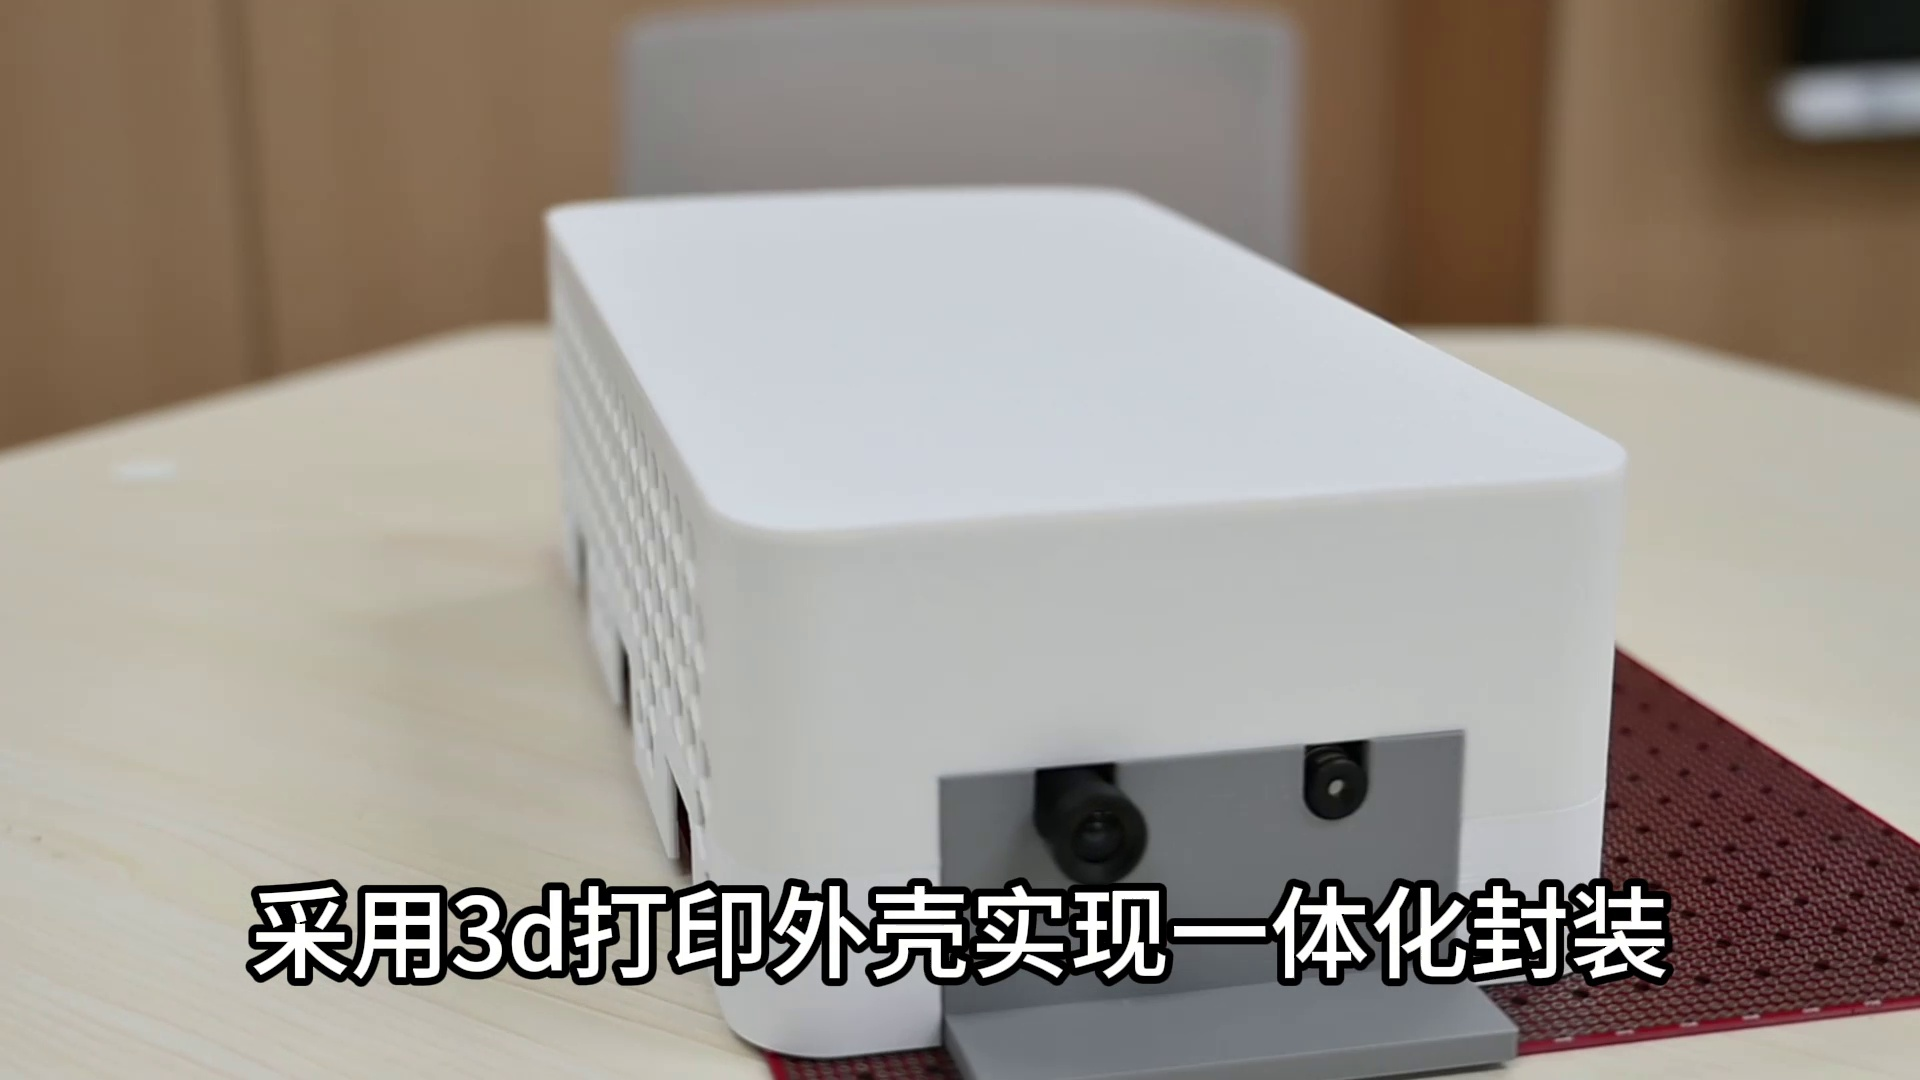
\includegraphics[width=.49\linewidth]{images/video-enclosure-front.jpg}\hfill
 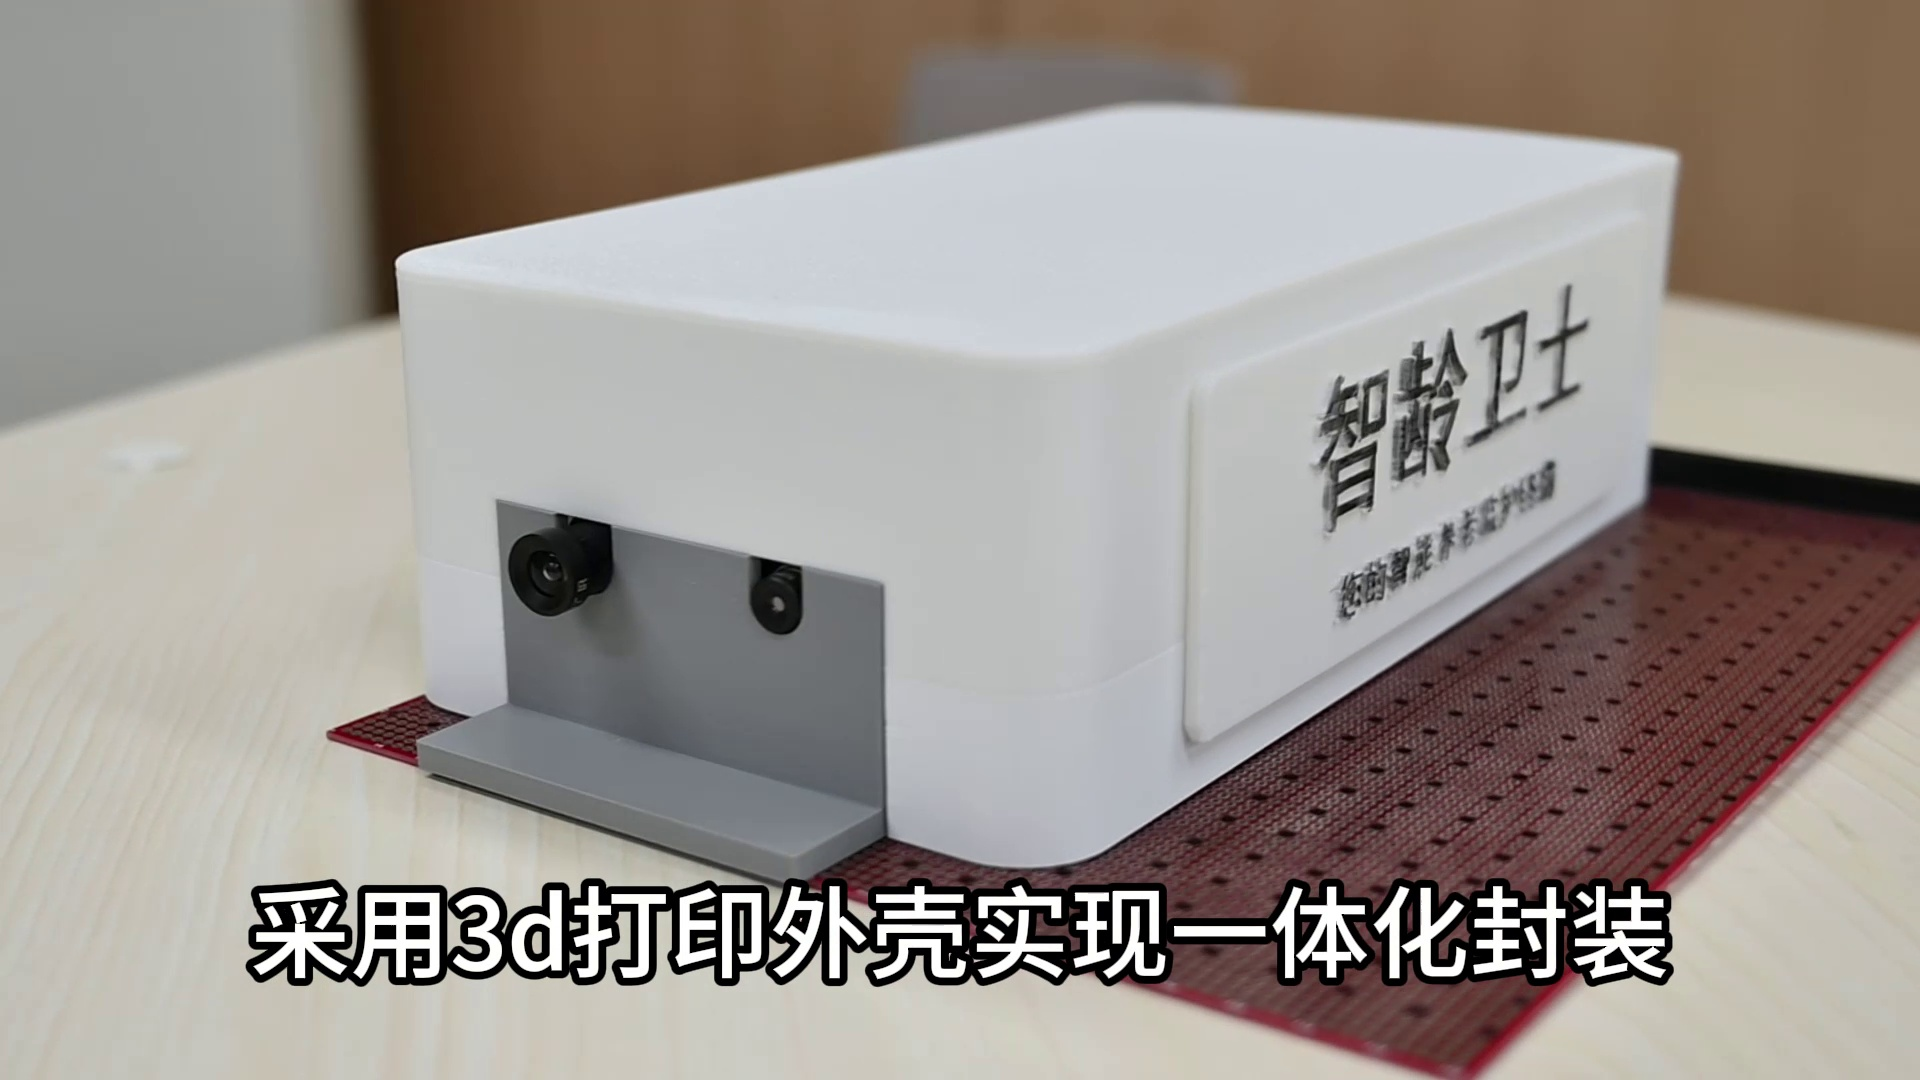
\includegraphics[width=.49\linewidth]{images/video-enclosure-oblique.jpg}
 \caption{终端正面与斜视实物}\label{fig:enclosure-views}
\end{figure}

\subsubsection{电路成果}
开发板、扩展子卡和外接线路的实物布局见图\ref{fig:hardware-video}，信号连接与引脚分配对应图\ref{fig:external-wiring}和表\ref{tab:external-pins}。原配摄像头排线、网线及USB连接保留，外接传感器和执行器通过扩展排针连接。

\begin{figure}[H]
 \centering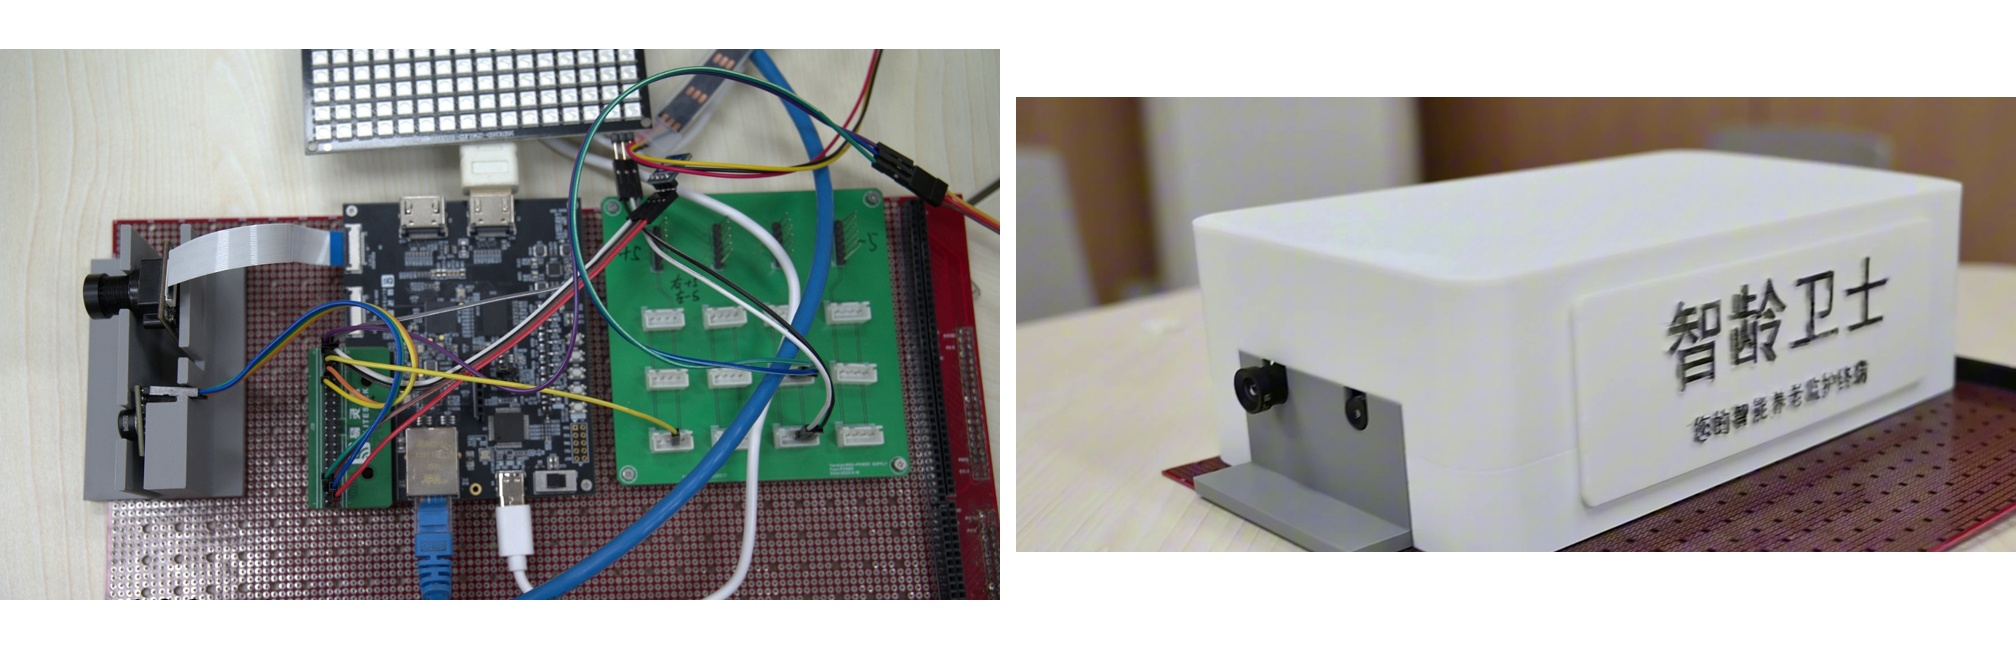
\includegraphics[width=\linewidth]{images/video-overview.jpg}
 \caption{开发平台与3D打印终端外壳}\label{fig:hardware-video}
\end{figure}

\subsubsection{软件成果}
Web界面见图\ref{fig:web-video}。实时区域显示预览、人员状态及环境数据，事件列表提供历史图像、记录及CSV导出，控制入口支持人工干预。板载HTTP提供状态与控制服务，电脑负责视频转换和数据库存档，使照护人员能够从当前风险追溯到对应事件。实时查看和历史复核共用目标及事件信息，连接异常发现与依据查看。

\begin{figure}[H]
 \centering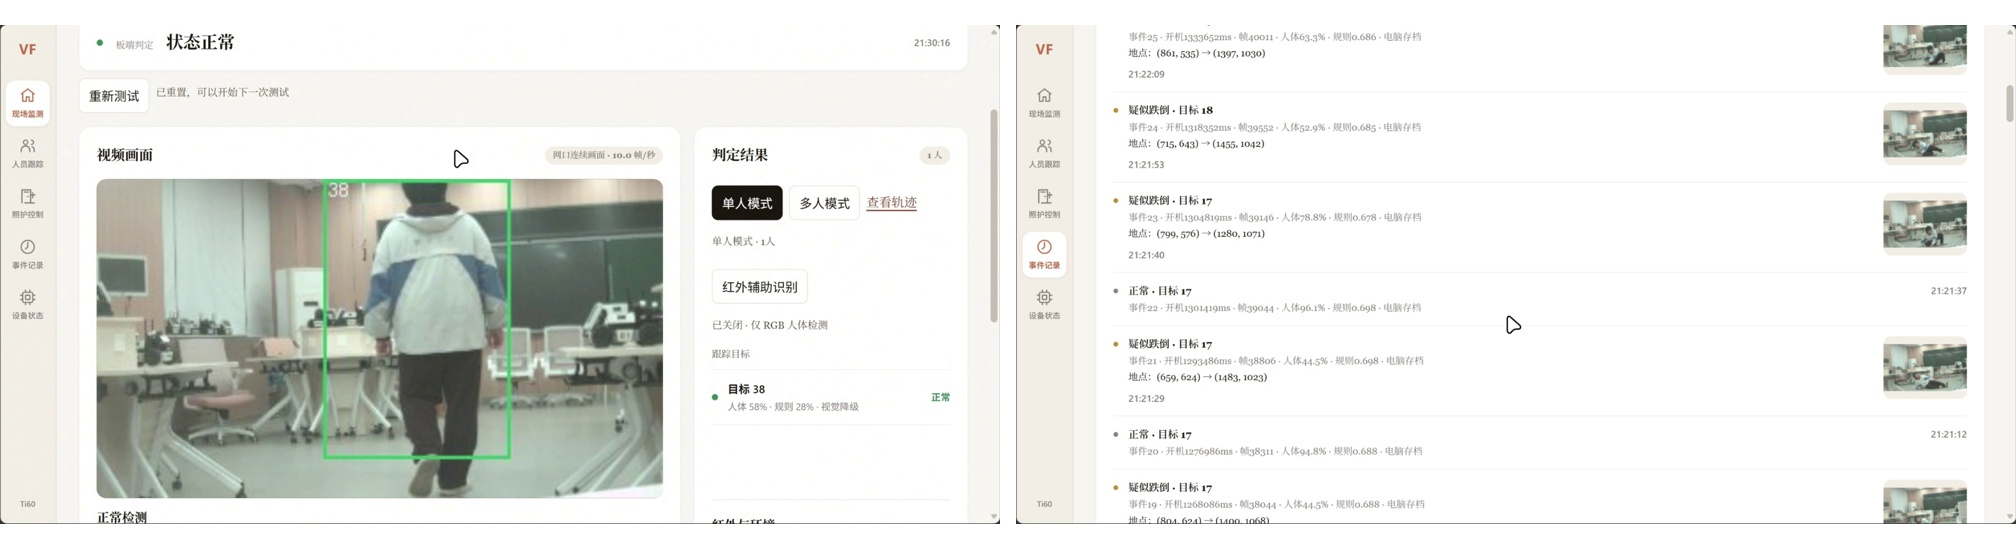
\includegraphics[width=\linewidth]{images/video-web.jpg}
 \caption{Web实时监控与历史事件界面}\label{fig:web-video}
\end{figure}

图\ref{fig:multi-video}中，两名人员同时位于监测区域，系统分别显示两个检测框。该结果说明当前场景下能够同时输出两个候选；长期身份保持及交叉遮挡表现另属跟踪性能评价。
\begin{figure}[H]
 \centering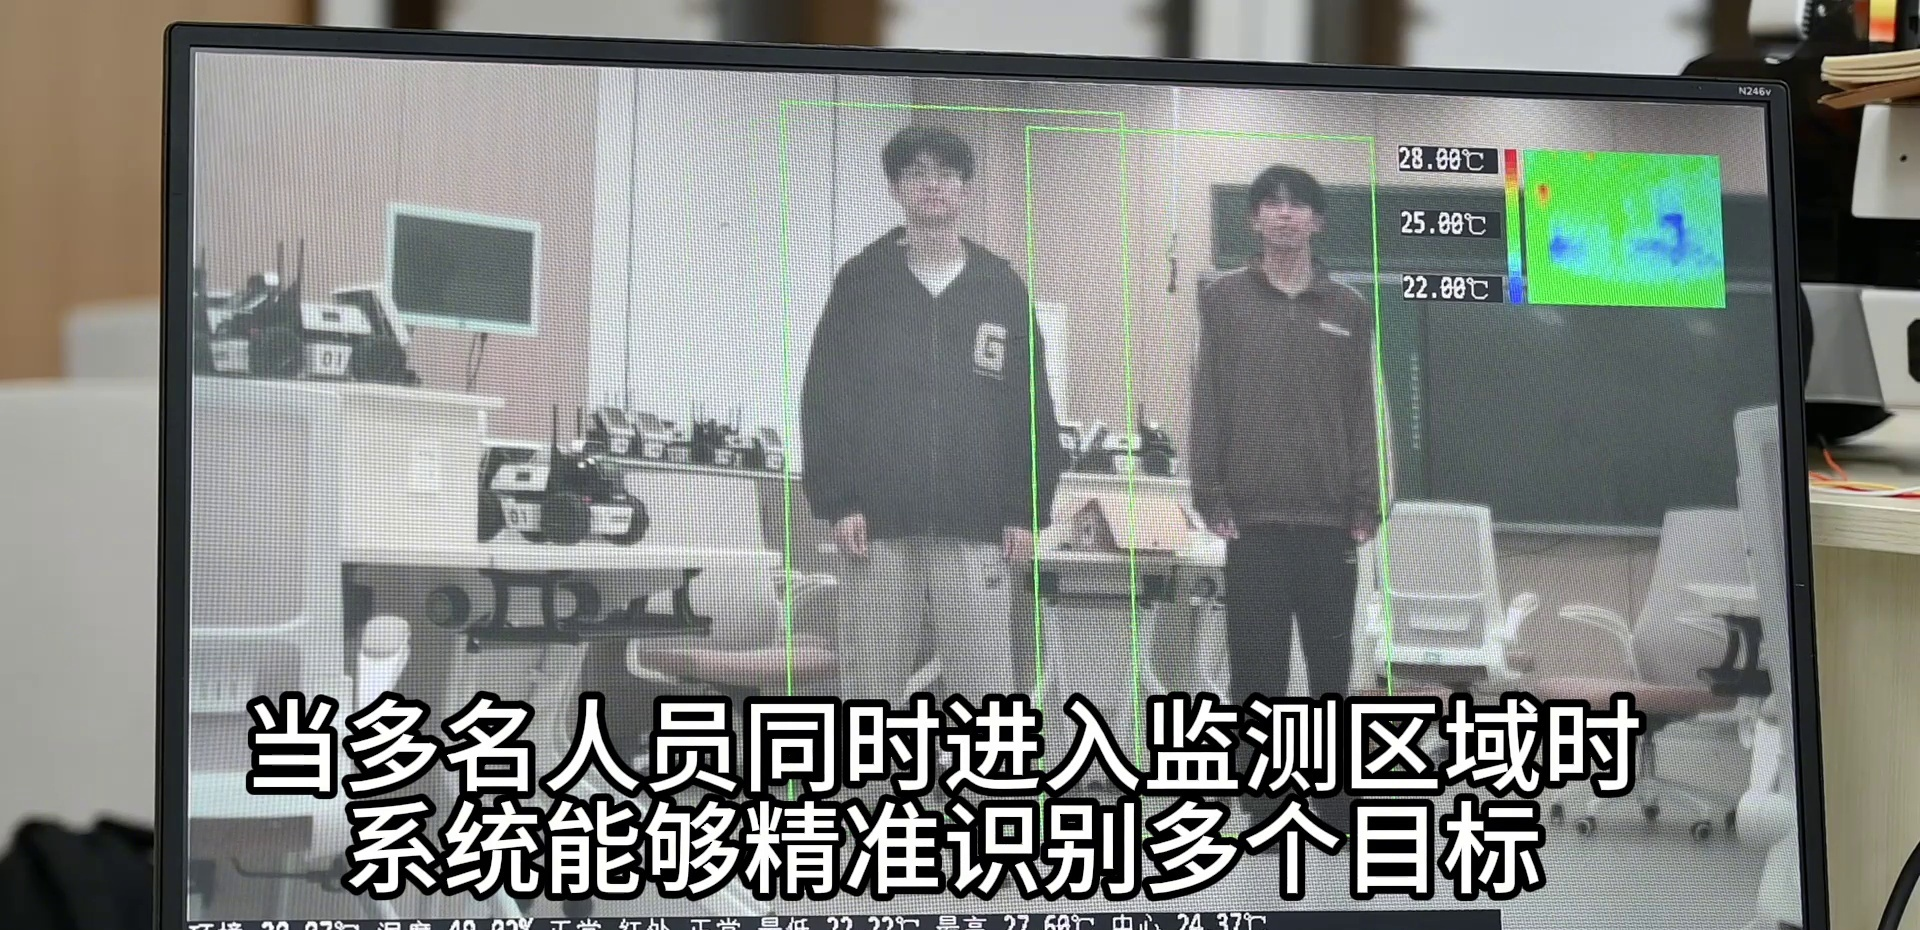
\includegraphics[width=.86\linewidth]{images/video-multi.jpg}
 \caption{多人目标检测画面}\label{fig:multi-video}
\end{figure}

\subsection{功能验证与结果分析}
\subsubsection{视觉候选与红外热观测}
人物照片与真人对照见图\ref{fig:photo-video}。一组画面中，照片的人体轮廓及纹理产生视觉候选，说明平面人物图像可以构成外观干扰；另一组画面中，真人保留检测框，照片未显示相同框。两组结果展示候选输出差异，尚不能单独确定变化由热辅助造成。表\ref{tab:ir-demo}区分各观测对象及结果意义。

\begin{figure}[H]
 \centering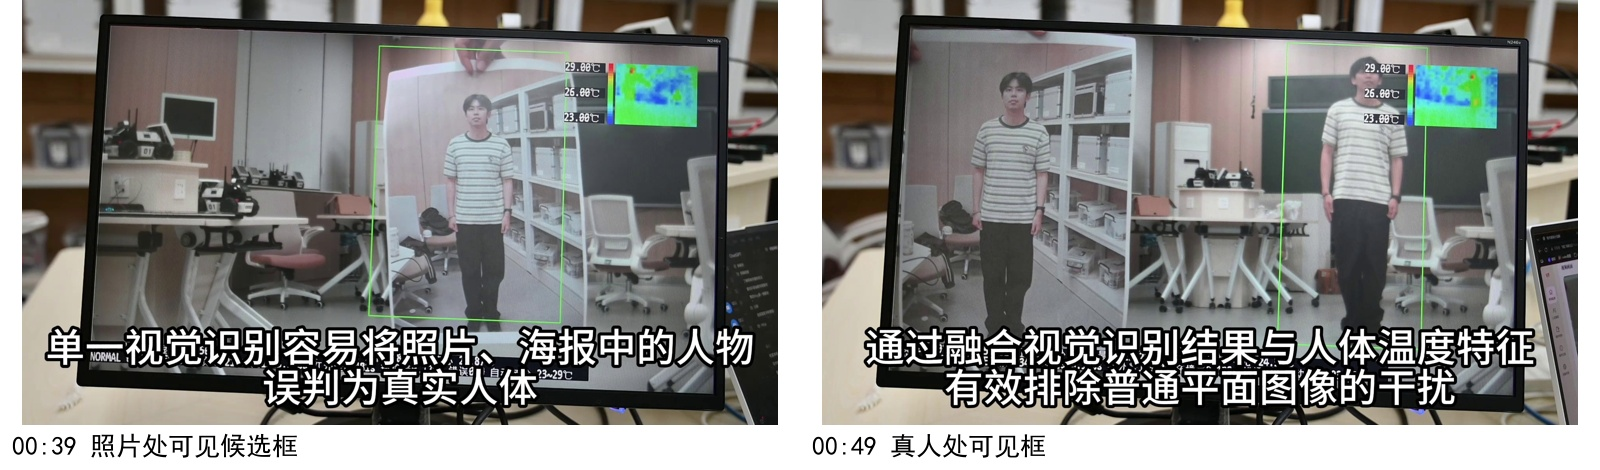
\includegraphics[width=\linewidth,trim=0 45bp 0 0,clip]{images/video-photo.jpg}
 \caption{人物照片与真人的检测画面对比}\label{fig:photo-video}
\end{figure}
\begin{table}[H]
 \centering\small
 \caption{视觉对照与热像观测结果}\label{tab:ir-demo}
 \begin{tabularx}{\linewidth}{@{}p{25mm}Y Y@{}}
 \toprule 观测对象 & 画面结果 & 结果说明 \\
 \midrule
 人物照片 & 人体外观可产生RGB候选 & 说明模型可能受平面图像干扰 \\
 真人对照 & 真人保留框，照片未显示相同框 & 展示候选差异，不能独立归因于热辅助 \\
 手部热像 & 手部与背景呈温度分布差异 & 说明阵列能显示区域热特征 \\
 \bottomrule
 \end{tabularx}
\end{table}

图\ref{fig:thermal-hand}为有手情况下的红外热成像画面。手部区域呈现较明显的暖色分布，与背景形成温度差异，说明阵列能够提供独立于可见光纹理的区域热观测。该结果验证热像采集与显示，目标级热确认仍依赖RGB与红外配准及对应区域查询。

\begin{figure}[H]
 \centering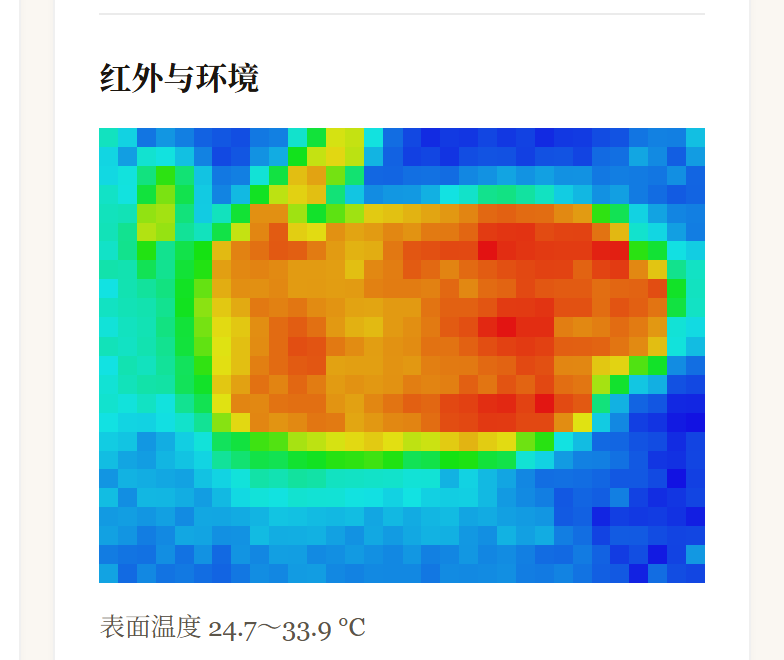
\includegraphics[width=.57\linewidth,height=66mm,keepaspectratio]{images/thermal-hand.png}
 \caption{有手情况下的红外热成像画面}\label{fig:thermal-hand}
\end{figure}

\subsubsection{正常与无人模式切换}
图\ref{fig:power-video}展示无人监视及人员重新入场两种状态。无人监视时，HDMI背景调暗，网页标示低功耗监视及2.0帧／秒；人员进入后，HDMI恢复正常亮度，网页显示10.0帧／秒。该现象与预览发送目标由2 FPS恢复至10 FPS的配置一致，接收端记录另呈现接近10、2、10 FPS的正常—无人—恢复变化。表\ref{tab:power-demo}给出模式配置，界面数值与接收端记录分别说明状态发布和网络预览变化。

\begin{figure}[H]
 \centering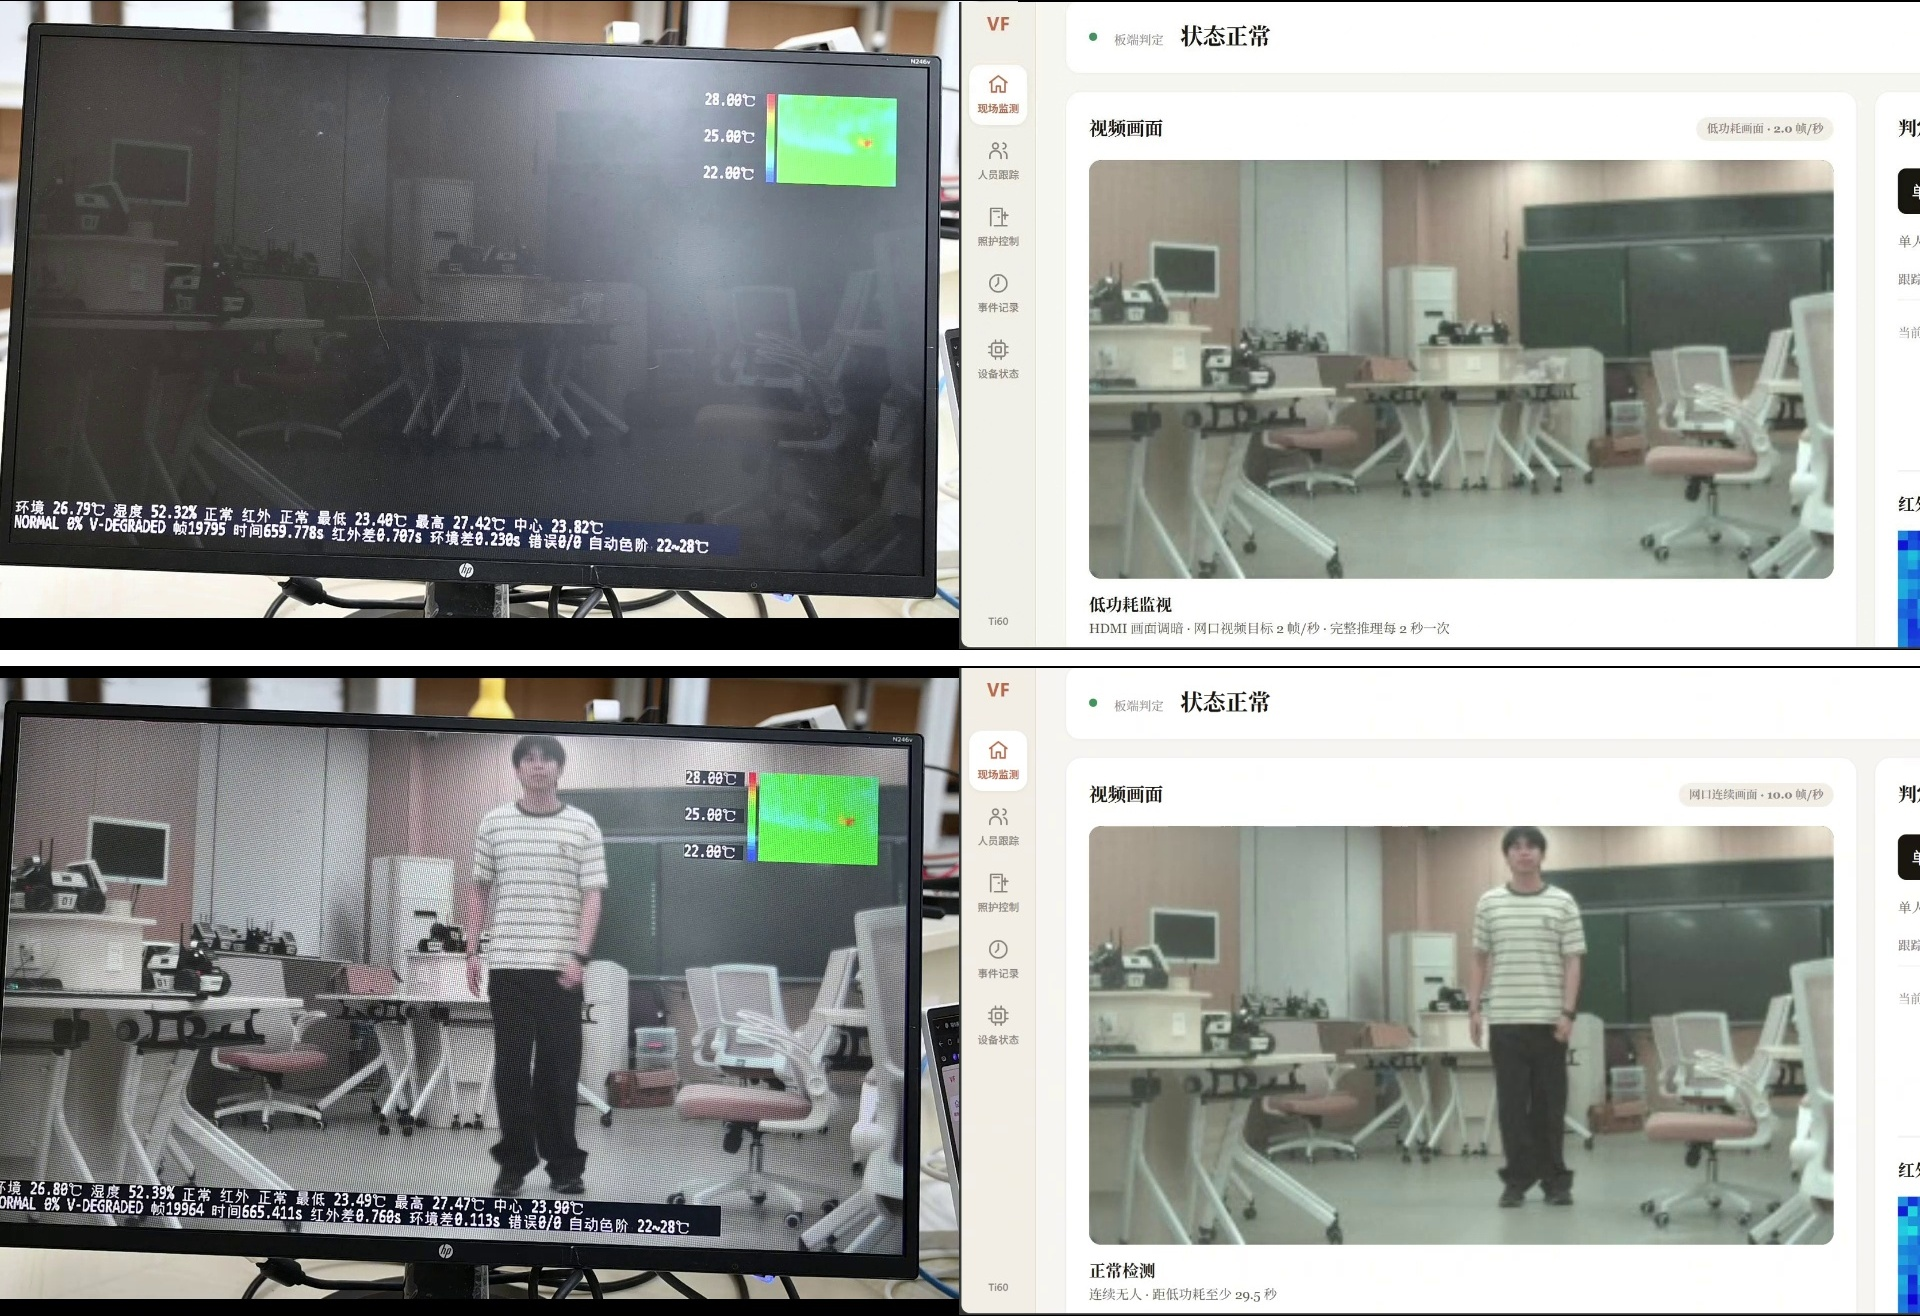
\includegraphics[width=\linewidth]{images/video-power.jpg}
 \caption{无人监视与人员入场后的HDMI及Web画面}\label{fig:power-video}
\end{figure}
\begin{table}[H]
 \centering\small
 \caption{正常、无人及恢复模式对照}\label{tab:power-demo}
 \begin{tabularx}{\linewidth}{@{}p{16mm}Y Y Y@{}}
 \toprule 模式 & HDMI背景 & 预览发送目标 & 检测与恢复策略 \\
 \midrule
 正常 & 正常背景 & 10 FPS & 正常完整推理调度 \\
 轻量监视 & RGB通道右移2位 & 2 FPS & 运动检查及2秒周期检测 \\
 入场恢复 & 恢复正常背景 & 10 FPS & 运动或候选唤醒，保持约10秒 \\
 \bottomrule
 \end{tabularx}
\end{table}

预览帧率描述网络图像更新频率，摄像头采集帧率与模型调用频率分别统计。采样窗$\Delta t$内，模型调用次数$\Delta N$和累计调用墙钟耗时$\Delta T_{\mathrm{invoke}}$可用于表征推理工作量：
\begin{equation}
 f_{\mathrm{infer}}=\frac{\Delta N}{\Delta t},\qquad
 R_{\mathrm{invoke}}=\frac{\Delta T_{\mathrm{invoke}}}{\Delta t}\times100\%.
 \label{eq:workload}
\end{equation}
式\eqref{eq:workload}分别表示模型调用频率及调用墙钟耗时占采样窗的比例，后者描述软件调用占用时间。现有结果支持无人切换、预览发送减少及入场恢复的功能关系；未给出同条件的调用次数对照与整机功率结果，因此不由背景调暗或预览降帧推导节电比例。

\clearpage
\subsubsection{正常蹲下与持续疑似跌倒}
动作场景以正常蹲下和持续近地姿态进行对照，结果见图\ref{fig:fall-video}。正常蹲下未直接触发红色预警，持续疑似先进入黄色观察，随后升级为红色并产生事件变化。这与先观察、后升级的状态设计一致，表\ref{tab:fall-demo}给出状态及处理规则。

\begin{figure}[H]
 \centering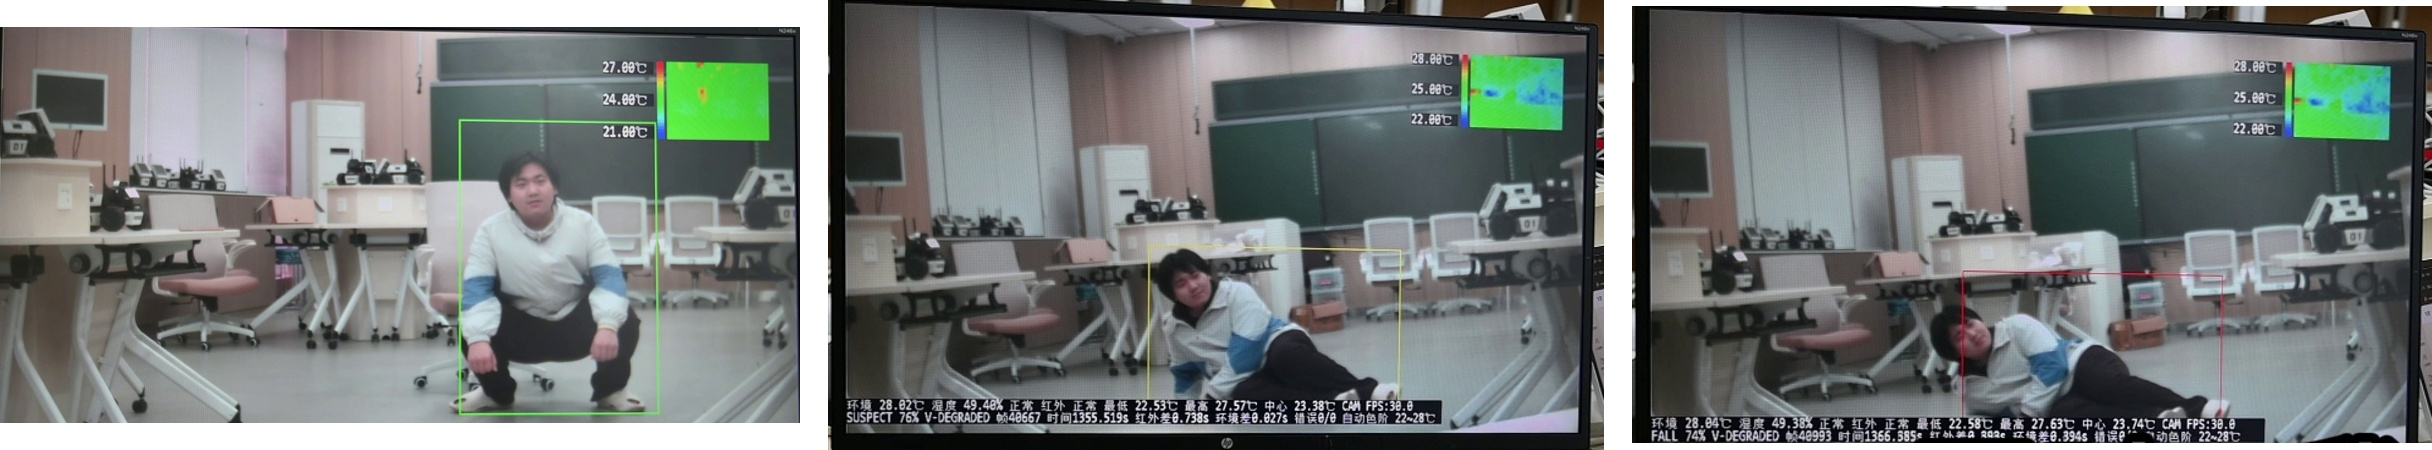
\includegraphics[width=\linewidth]{images/video-fall.jpg}
 \caption{正常蹲下、黄色疑似与红色预警画面对比}\label{fig:fall-video}
\end{figure}
\begin{table}[H]
 \centering\small
 \caption{动作场景与状态处理}\label{tab:fall-demo}
 \begin{tabularx}{\linewidth}{@{}p{22mm}Y Y@{}}
 \toprule 场景 & 状态特征 & 处理机制 \\
 \midrule
 正常蹲下 & 演示中未直接升级为红色 & 结合历史框形与运动继续判断 \\
 持续疑似 & 黄色观察后升级为红色 & 同ID持续计时与风险升级 \\
 恢复直立 & 持续满足恢复条件 & 返回正常并清除疑似计时 \\
 目标切换或长间断 & 目标历史连续性中断 & 重新建立对应计时 \\
 人工干预 & 停止动作或重置监测 & 分别处理执行器与风险状态 \\
 \bottomrule
 \end{tabularx}
\end{table}

该场景说明系统没有将所展示的短暂蹲下直接处理为红色预警，并能对持续疑似完成升级。\textbf{10秒为同一目标疑似持续门槛，不是实测端到端报警时延}；响应还受模型调用间隔、状态进入条件及服务调度影响。持续蹲姿、遮挡和ID切换仍可能影响结果，误报与漏报需按完整事件统计。

\subsubsection{消息提示与模拟门响应}
图\ref{fig:response-video}展示风险状态与模拟门动作。板端发布红色事件后，RISC-V照护模块发送执行命令，FPGA输出舵机控制波形，完成模拟门响应。电脑消息服务读取事件并调用QQ接口，Web提供实时状态和历史查看。执行、通知与复核以同一风险事件关联，分别承担现场动作、远程提示和人工判断。

\begin{figure}[H]
 \centering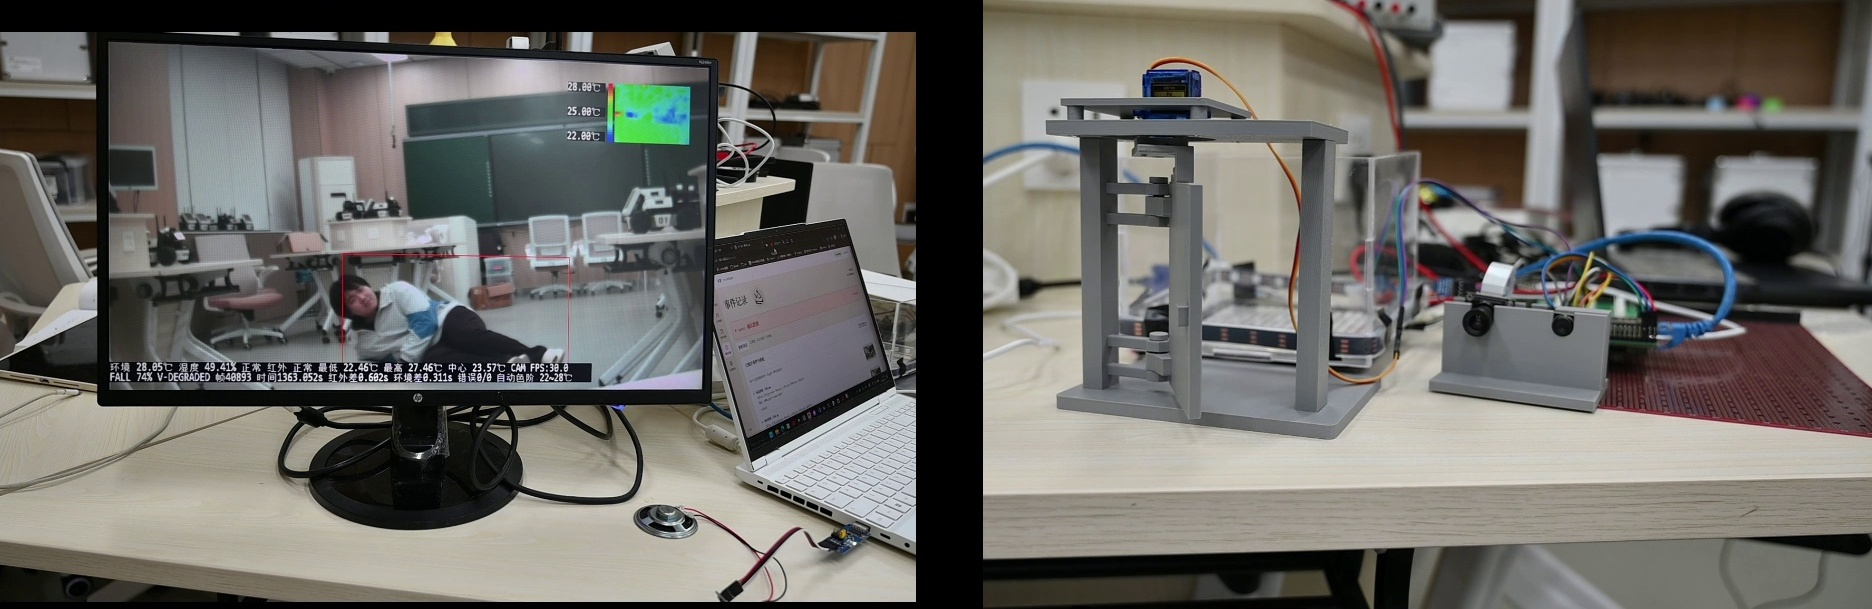
\includegraphics[width=.9\linewidth]{images/video-response.jpg}
 \caption{风险显示与模拟门联动画面}\label{fig:response-video}
\end{figure}

当前视觉风险、照护报警锁存及执行器运动分别管理：风险可以恢复，锁存用于避免重复动作，人工取消停止后续运动，重新监测清理人员历史。演示呈现了风险显示、QQ报警记录与机构动作，完整通知链时延、语音实播及长期稳定性仍需分别测量；真实设施还需限位、防夹及故障保护。

\subsubsection{国产大模型DeepSeek接入与照护问答}
系统通过电脑端消息桥接接入国产大模型DeepSeek，以QQ作为手机端照护问答入口。用户提问转入DeepSeek对应会话，生成答复后返回QQ，形成“手机提问—消息桥接—模型生成—手机答复”的交互链路。

图\ref{fig:activity-chat}展示“今天老人活动状况怎么样？”的问答，答复概述活动区域并建议联系关怀。\textbf{板端承担实时风险判断，DeepSeek承担自然语言交互}；检测、持续计时和模拟门控制在本地运行。该设计将固定报警扩展为可对话的远程照护服务。

针对按日活动查询，模型先读取真实采样汇总，再依据已观测区域生成活动概述和联系关怀建议。\textbf{“未记录到某房间”不等于“全天没有去过”}；无有效记录时明确返回数据不足。统计只覆盖采集程序运行、地面标定有效且主目标可见的时段，目标ID不承担身份识别。问答画面用于展示交互形式，不作为全天统计准确性或食欲、疾病推断的验证结果。

\begin{figure}[H]
 \centering
\includegraphics[width=.63\linewidth]{images/video-activity-chat-redacted.png}
 \caption{接入DeepSeek的手机端照护问答界面}\label{fig:activity-chat}
\end{figure}

\subsubsection{位置映射与灯光表达}
位置显示以选定目标的地面映射点为输入，在16×16矩阵上表达当前位置与短时轨迹，并根据相对墙距选择区域灯光。图\ref{fig:trajectory-video}中，人员在标定范围内行走，网页地图与实体灯板显示相应的位置及轨迹变化。两种显示读取同一归一化位置与轨迹状态，分别面向浏览器查看和现场提示。
\begin{figure}[H]
 \centering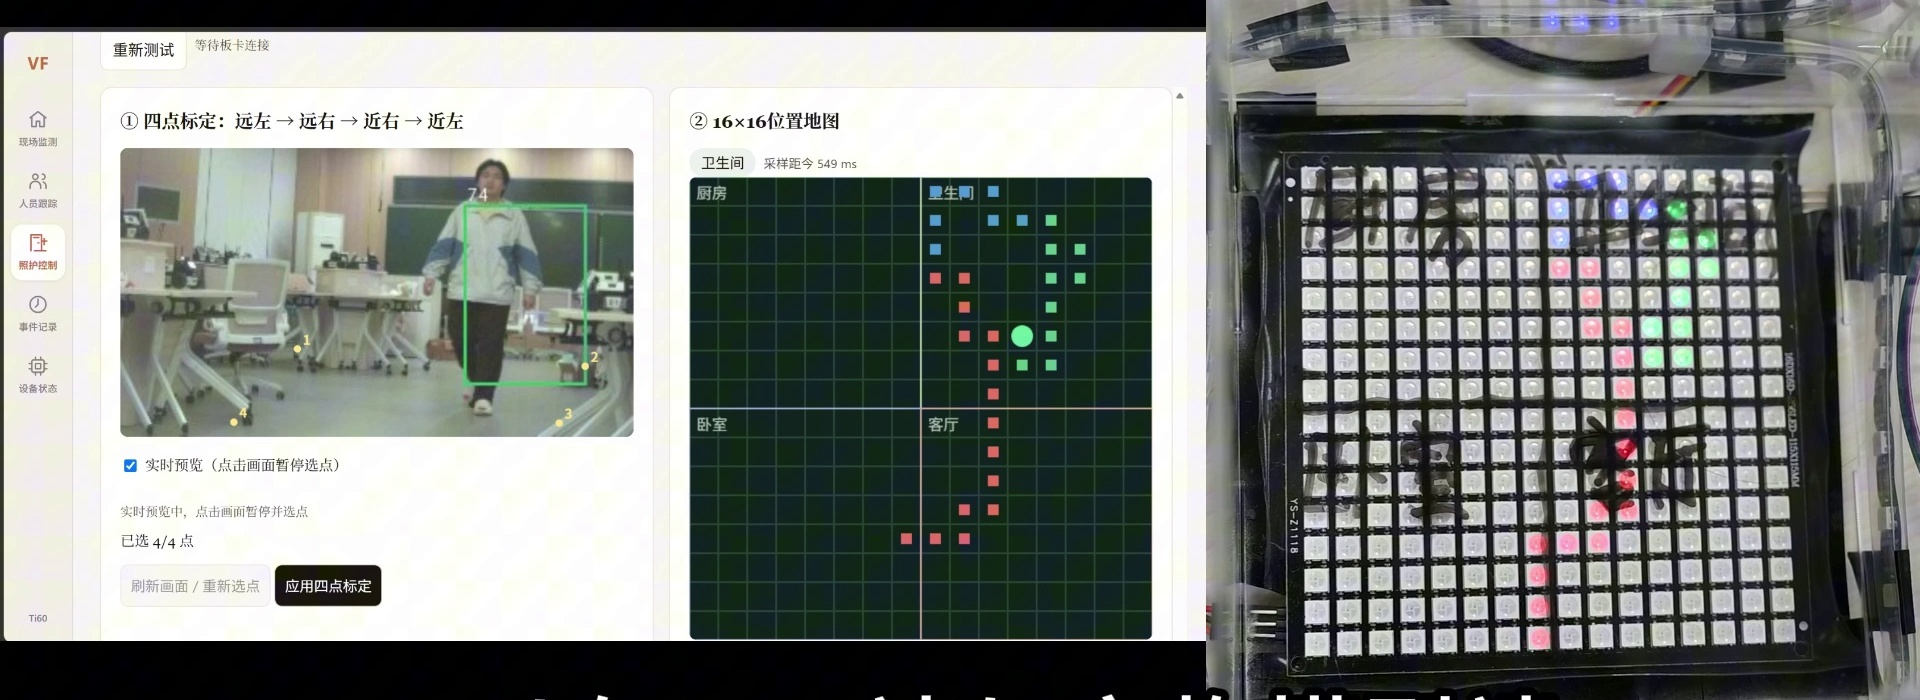
\includegraphics[width=\linewidth]{images/video-trajectory.jpg}
 \caption{网页地图与实体灯板的轨迹显示}\label{fig:trajectory-video}
\end{figure}

\begin{samepage}
轨迹按经过时间依次显示为绿色、蓝色和红色，每一颜色阶段为3秒，累计9秒后清除。\textbf{轨迹颜色表示历史新旧，风险框颜色表示异常阶段}，二者使用不同语义。红色风险通过外墙灯闪烁提示，位置与灯光的数据关系见图\ref{fig:led-map}。
\par
\end{samepage}

\begin{figure}[H]
 \centering
 \begin{tikzpicture}
  \node[block,text width=40mm] (a) at (0,0) {人员框底边中心\\四点地面映射};
  \node[block,text width=40mm] (b) at (5.8,0) {归一化平面位置\\有效性与目标ID检查};
  \node[block,text width=40mm] (c) at (0,-1.7) {16×16矩阵位置\\连续轨迹与颜色老化};
  \node[block,text width=40mm] (d) at (5.8,-1.7) {最近墙方向联动\\红色风险触发外墙闪烁};
  \node[block,text width=75mm] (e) at (2.9,-3.4) {DDR灯帧暂存与握手供数\\FPGA串行波形输出};
  \draw[flow] (a)--(b);
  \draw[flow] (b.south)--++(0,-.25)-|(c.north);
  \draw[flow] (b)--(d);
  \draw[flow] (c.south)--++(0,-.25)-|(e.north);
  \draw[flow] (d.south)--++(0,-.25)-|(e.north);
 \end{tikzpicture}
 \caption{位置映射与灯光联动原理}\label{fig:led-map}
\end{figure}

位置映射依赖固定机位及地面平面假设，移动支架后需重新标定。目标切换或位置失效时中断补线，避免将不同人员或无效位置连接为同一轨迹。行走演示说明位置到网页及实体输出的功能通路，定位误差与显示时延仍需按已知地面点测量；位置显示以选定主目标为对象，多人轨迹记录不等同于为所有人员独立驱动一套照护输出。

\subsection{资源使用与性能分析}
\subsubsection{硬件资源与时序}
表\ref{tab:resources}给出已完成硬件实现的资源及静态时序。XLR和片内RAM分别占98.87\%与99.61\%，构成后续拓展的主要约束；DSP占46.88\%，仍有算术资源余量。灯帧与事件使用DDR组织，以适应片内存储紧张的条件。
\begin{table}[H]
 \centering\small
 \caption{硬件资源占用与静态时序结果}\label{tab:resources}
 \begin{tabularx}{.94\linewidth}{@{}*{4}{>{\centering\arraybackslash}X}@{}}
 \toprule 指标 & 已用 & 总量 & 占用或结果 \\
 \midrule
 XLR & 60,114 & 60,800 & 98.87\% \\
 片内RAM块 & 255 & 256 & 99.61\% \\
 DSP & 75 & 160 & 46.88\% \\
 最小建立余量 & \multicolumn{2}{c}{0.260 ns} & 正余量 \\
 最小保持余量 & \multicolumn{2}{c}{0.026 ns} & 正余量 \\
 \bottomrule
 \end{tabularx}
\end{table}

最小建立余量为0.260 ns，最小保持余量为0.026 ns，说明该实现在所用约束下通过建立和保持检查；较小余量也限制继续增加关键路径逻辑。资源表反映整套硬件，不能单独量化DDR灯帧节省的片内RAM。存储组织可由1,152字节DDR数组及握手输出说明，性能收益需用同条件实现对照评价。

\subsubsection{系统拓展与协同关系}
围绕赛题的多模态智能终端方向\cite{guide}，作品连接本地决策、多人检测、事件存档、无人调度与照护输出，模块作用见表\ref{tab:extension-status}。实时风险由板端产生，预览转换、历史数据库及外部消息依赖电脑辅助程序，该分工决定了现场监测与远程服务各自的运行条件。
\begin{table}[H]
 \centering\small
 \caption{系统拓展与协同功能}\label{tab:extension-status}
 \begin{tabularx}{\linewidth}{@{}p{25mm}Y Y@{}}
 \toprule 模块 & 主要实现 & 系统作用 \\
 \midrule
 事件上报与复核 & 同帧缩略图、确认队列、入库及去重 & 保存触发依据，支持历史查看 \\
 RISC-V本地决策 & 模型调度、同ID规则及照护控制 & 在板端形成风险与响应状态 \\
 多目标管理 & IOU关联与16槽历史 & 连接多个人员的短时观测 \\
 无人场景调度 & 推理、背景与10／2 FPS预览协同 & 减少无人时的冗余工作 \\
 Web与智能交互 & HTTP、SQLite、QQ及DeepSeek会话 & 实时查看、事件复核、远程报警及照护问答 \\
 UART语音 & CRC、时效保护及电脑串口桥接 & 将有效红色状态转换为语音指令 \\
 位置灯板与外墙灯 & 地面映射、轨迹与DDR流式输出 & 表达位置并提供现场风险提示 \\
 \bottomrule
 \end{tabularx}
\end{table}

\subsubsection{评价范围与适用条件}
现阶段结果包括双人候选显示、黄色至红色的分阶段预警、Web复核、无人模式切换、模拟门控制、网页与实体轨迹显示，以及手机活动问答。\textbf{RGB与红外空间配准尚未完成，热辅助候选确认和风险分支尚不具备目标级效果评价条件}；热像显示不能作为照片过滤成功的充分证据。位置跟随误差、全天活动统计准确性、语音实播、完整通知链时延及连续运行稳定性仍需专项验证。

检测性能可采用精确率和召回率评价：
\begin{equation}
 \mathrm{Precision}=\frac{TP}{TP+FP},\qquad
 \mathrm{Recall}=\frac{TP}{TP+FN}.
 \label{eq:metrics}
\end{equation}
其中$TP$、$FP$、$FN$分别为正确检测、误检与漏检数量，检测框匹配采用统一IoU条件。人员和场景应在训练与测试之间独立划分，跌倒评价以完整事件为单位，统计事件召回率、单位观察时长误报次数和响应时延。现阶段结果以功能验证为主，尚未形成独立数据集上的P、R、mAP及误报率统计，也未完成整机功率测量。

全视场输入在覆盖范围与远处目标细节之间取舍，持续观察在判定稳定性与响应等待之间取舍；轻量监视还需兼顾唤醒开销、入场检测及功率变化。因此，现阶段结果定位于固定室内场景下的系统功能验证，尚不能外推为任意人群、距离和环境下的识别或节能性能。

\FloatBarrier
\clearpage
\section{总结}
\subsection{可扩展之处}
后续首先完善目标级辅助感知：完成固定机位下的近距离RGB与红外配准，评价照片辅助筛选与远距离纯视觉监测效果，验证热信息不足时的视觉回退。其次完善目标与风险评价，增加人员交叉、持续蹲姿和短时遮挡场景，按独立完整事件统计召回、误报和响应时延，分析持续门槛的取舍。

资源方面，结合赛题小模型建议\cite{guide}压缩模型及输入通路开销，对DDR供数和片内缓存开展同条件比较；调度方面，同步记录推理次数、预览发送量及整机功率，评价无人策略的收益与唤醒代价。系统方面，完善标定参数持久保存、通知回执、语音反馈和执行机构保护，并开展连续运行验证。

\subsection{心得体会}
本作品在Ti60 FPGA与RISC-V平台上完成了从全视场图像输入、INT8人体检测、目标历史到分阶段预警及模拟照护响应的集成。实物结果展示了双人检测、蹲下与持续疑似的不同处理、无人调暗与入场恢复，以及Web事件复核、QQ报警和模拟门联动。四点映射连接网页地图与实体灯板的轨迹显示，国产大模型DeepSeek经QQ消息桥接提供手机端照护问答，扩展了智能家居场景下的信息获取方式。硬件实现的建立及保持时序余量均为正。

开发中的主要体会是，模型输出需经过目标关联、持续状态及事件管理，才能形成可解释的照护响应。FPGA承担连续像素和波形，RISC-V承担历史与控制，电脑扩展存档及通知，明确分工便于在有限资源内形成完整流程。后续将重点完善目标级热配准、独立事件统计和整机能效测量，提高实际照护所需的可靠性。

\clearpage
\section{参考文献}
\begingroup
\renewcommand{\section}[2]{}
\small
\begin{thebibliography}{9}
\setlength{\itemsep}{0pt}
\bibitem{board} TI60F225I3-V4 DEMO板软硬件设计说明[Z]. 260920版.
\bibitem{camera} 思特威. SC431HAI数据手册[Z]. V1.1, 2024-08-16.
\bibitem{tinyml} 易灵思（深圳）科技有限公司. TinyML User Guide（Draft）[Z]. UG-TinyML, V2.0, 2024-05-20.
\bibitem{iou} BOCHINSKI E, et al. IOU Tracker[CP/OL]. [2026-11-03]. \url{https://github.com/bochinski/iou-tracker}.
\bibitem{syn} 北京宇音天下科技有限公司. SYN6288中文语音合成芯片数据手册[Z]. 2011-09-06更新.
\bibitem{guide} 全国大学生嵌入式芯片与系统设计竞赛组委会. 2026 FPGA赛道选题指南：易灵思[Z]. 赛题三：多模态AI智能终端，第9—11页.
\bibitem{video} 团队. 室内照护终端功能演示[Z]. 2026.
\bibitem{project} 团队. 多模态室内照护终端软硬件设计与实现[Z]. 2026.
\end{thebibliography}
\endgroup
\end{document}
